\chapter{Aspectos gerais de ciências de dados}
\label{cap:background}

\section{O que é ciência de dados?}
%- Definir o que é ciência de dados
%https://docplayer.com.br/28263393-Introducao-a-ciencia-de-dados-mineracao-de-dados-e-big-data.html
% MARAL, F. \textbf{Introdução à Ciência de Dados:} Mineração de Dados e Big Data. 1. ed. Rio de Janeiro: Alta Books, 2016.

A ciência de dados é uma ciência nova, apesar da expressão \textit{Data Science} ser utilizada desde 1960. Ela é responsável por todo o ciclo de vida do dado, desde a coleta até o descarte, obtendo assim conhecimento e informação sobre ele ao longo deste ciclo. 

Com o intuito de obter resultados para tomadas de decisões, e por esses dados coletados geralmente serem volumosos e extraídos de várias fontes, é utilizado ferramentas, técnicas, modelos e processos. Estes meios comumente são derivados de outras áreas do conhecimento, como por exemplo, mineração de dados, estatística, \textit{big data}.


Um exemplo de processo comum na área de dados é o pipeline chamado ETL (Extrair, Transformar e Carregar). Esse pipeline move e transforma informações de diferentes fontes de dados em um ambiente de armazenamento centralizado. O ETL é extensamente utilizado na carreira de dados.

O cientista de dados é responsável por cuidar de todo o ciclo de vida da ciência de dado. De acordo com a figura \ref{fig:enter-labeldado2} o ciclo cobre desde o entendimento do problema, passando pela coleta, processamento e exploração dos dados, seguido da comunicação dos resultados e feedback \cite{Amaranta}. Esse profissional pode ter origem acadêmica ou empresarial e é cobrado dele uma visão sistemática, conhecimentos matemáticos, que podem ser de estatística ou de álgebra linear, além de linguagens de software. Ele consegue transformar o dado, que é a matéria-prima crua, em informação, onde o dado é analisado e atribuido um significado, e a informação em conhecimento, pois foi incumbido uma interpretação que foi entendida e aplicada para um fim. 

    \begin{figure}[!ht]
        \centering
        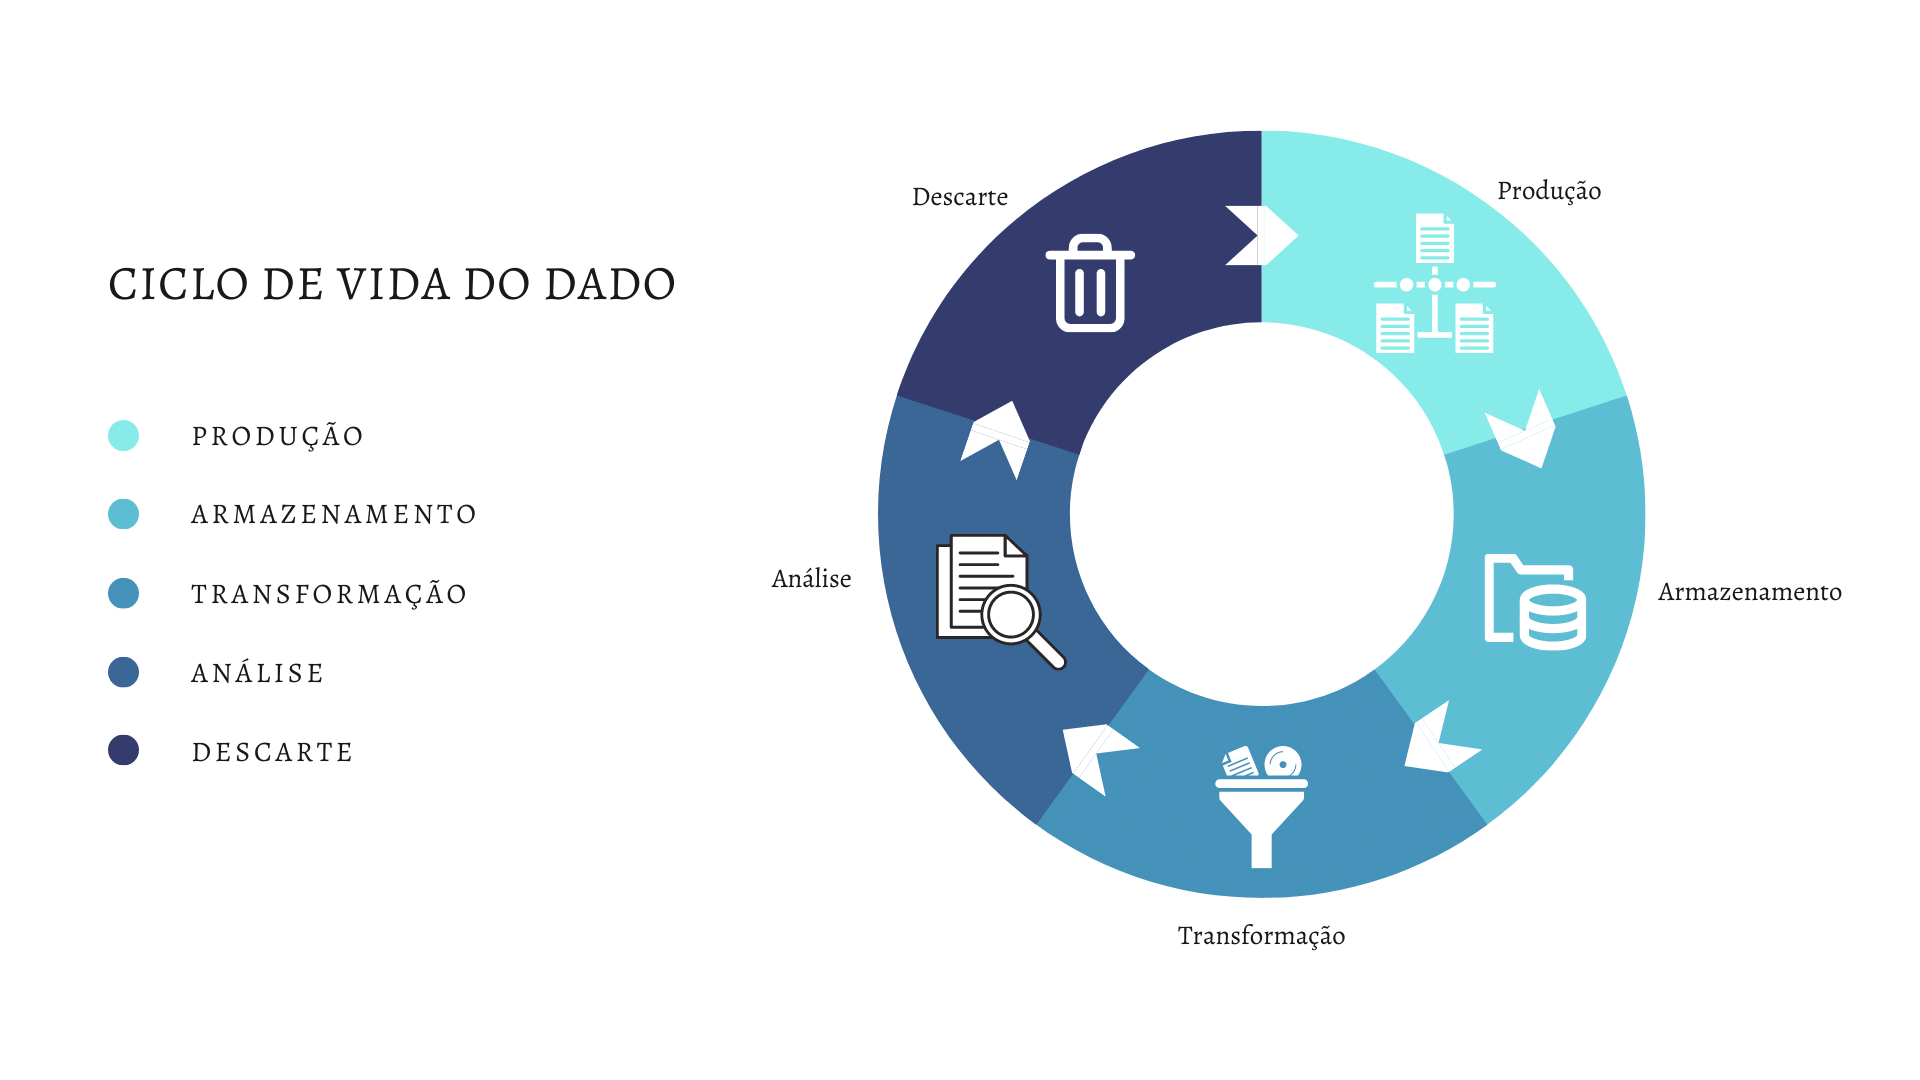
\includegraphics[width=0.9\linewidth]{fig/Capitulo2/1.png}
        \caption{Ciclo de Vida do Dado}
        \label{fig:enter-labeldado1}
    \end{figure}

    \begin{figure}[!ht]
        \centering
        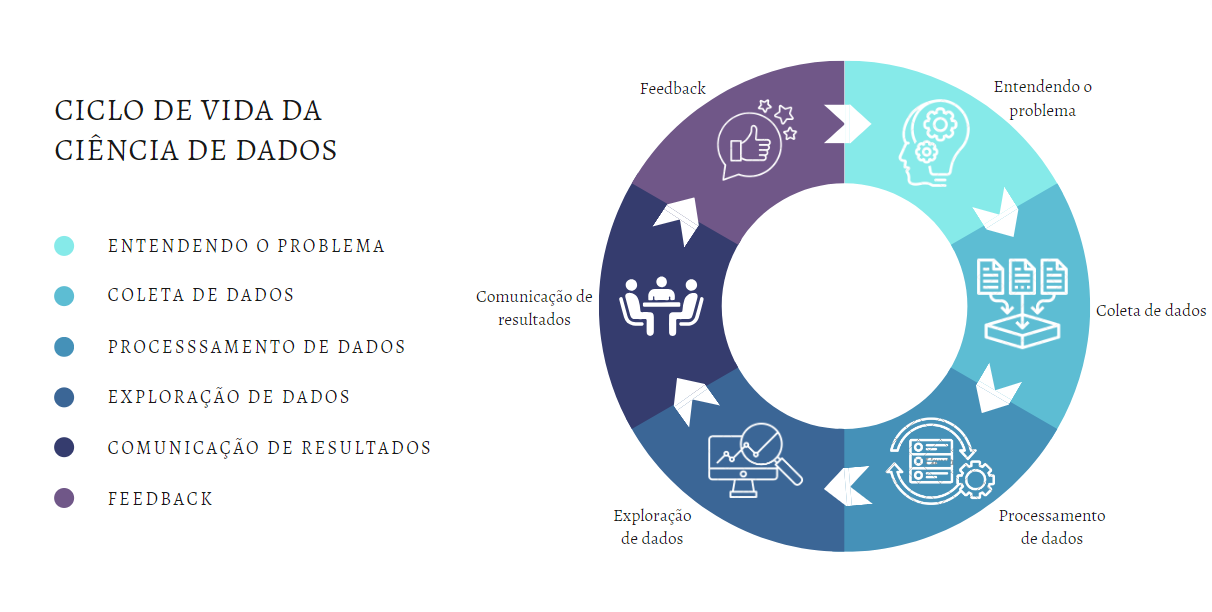
\includegraphics[width=0.9\linewidth]{fig/Capitulo2/2.png}
        \caption{Ciclo de vida da Ciência de Dados}
        \label{fig:enter-labeldado2}
    \end{figure}

\newpage

\section{Algoritmos de modelagem}
\subsection{Algoritmos de aprendizado de máquina}

Assim como os bebês aprendem através da repetição de palavras por seus pais quando estão aprendendo a falar, as máquinas aprendem através da repetição também. Elas possuem algoritmos com um grande volume de dados e algumas camadas de treinamento. Esses algoritmos são os de aprendizado de máquina (\textit{machine learning}).

Há 3 categorias de algoritmos, aprendizagem supervisionada, aprendizagem não supervisionada e aprendizagem por reforço. Cada uma é utilizada com tipos de dados e objetivos diferentes. Aqui será abordado definições focadas nos algoritmos de aprendizagem supervisionada pois foi desta categoria que foi encontrado no mapeamento sistemático a maioria dos modelos, e um deles será utilizado no final do trabalho para a implementação de um modelo de predição de óbitos no Estado de Goiás.

 \subsection{Algoritmos de Aprendizagem Supervisionada}

Esse algoritmo é alimentado com pares de entradas e saídas rotuladas e depois da fase de treinamento e teste, ele determina uma forma de prever as saídas baseando-se nas entradas fornecidas.

        \subsubsection{Algoritmos de classificação}

Quando os dados fornecidos são dados discretos, o aprendizado supervisionado age como um classificador, reconhecendo padrões desses dados e predizendo categorias para cada um deles.

    \subsubsection{Algoritmos de regressão}

Quando os dados fornecidos são dados contínuos, o algoritmo estuda as relações entre esses dados e é utilizado para prever resultados.


\begin{figure}[!ht]
    \centering
    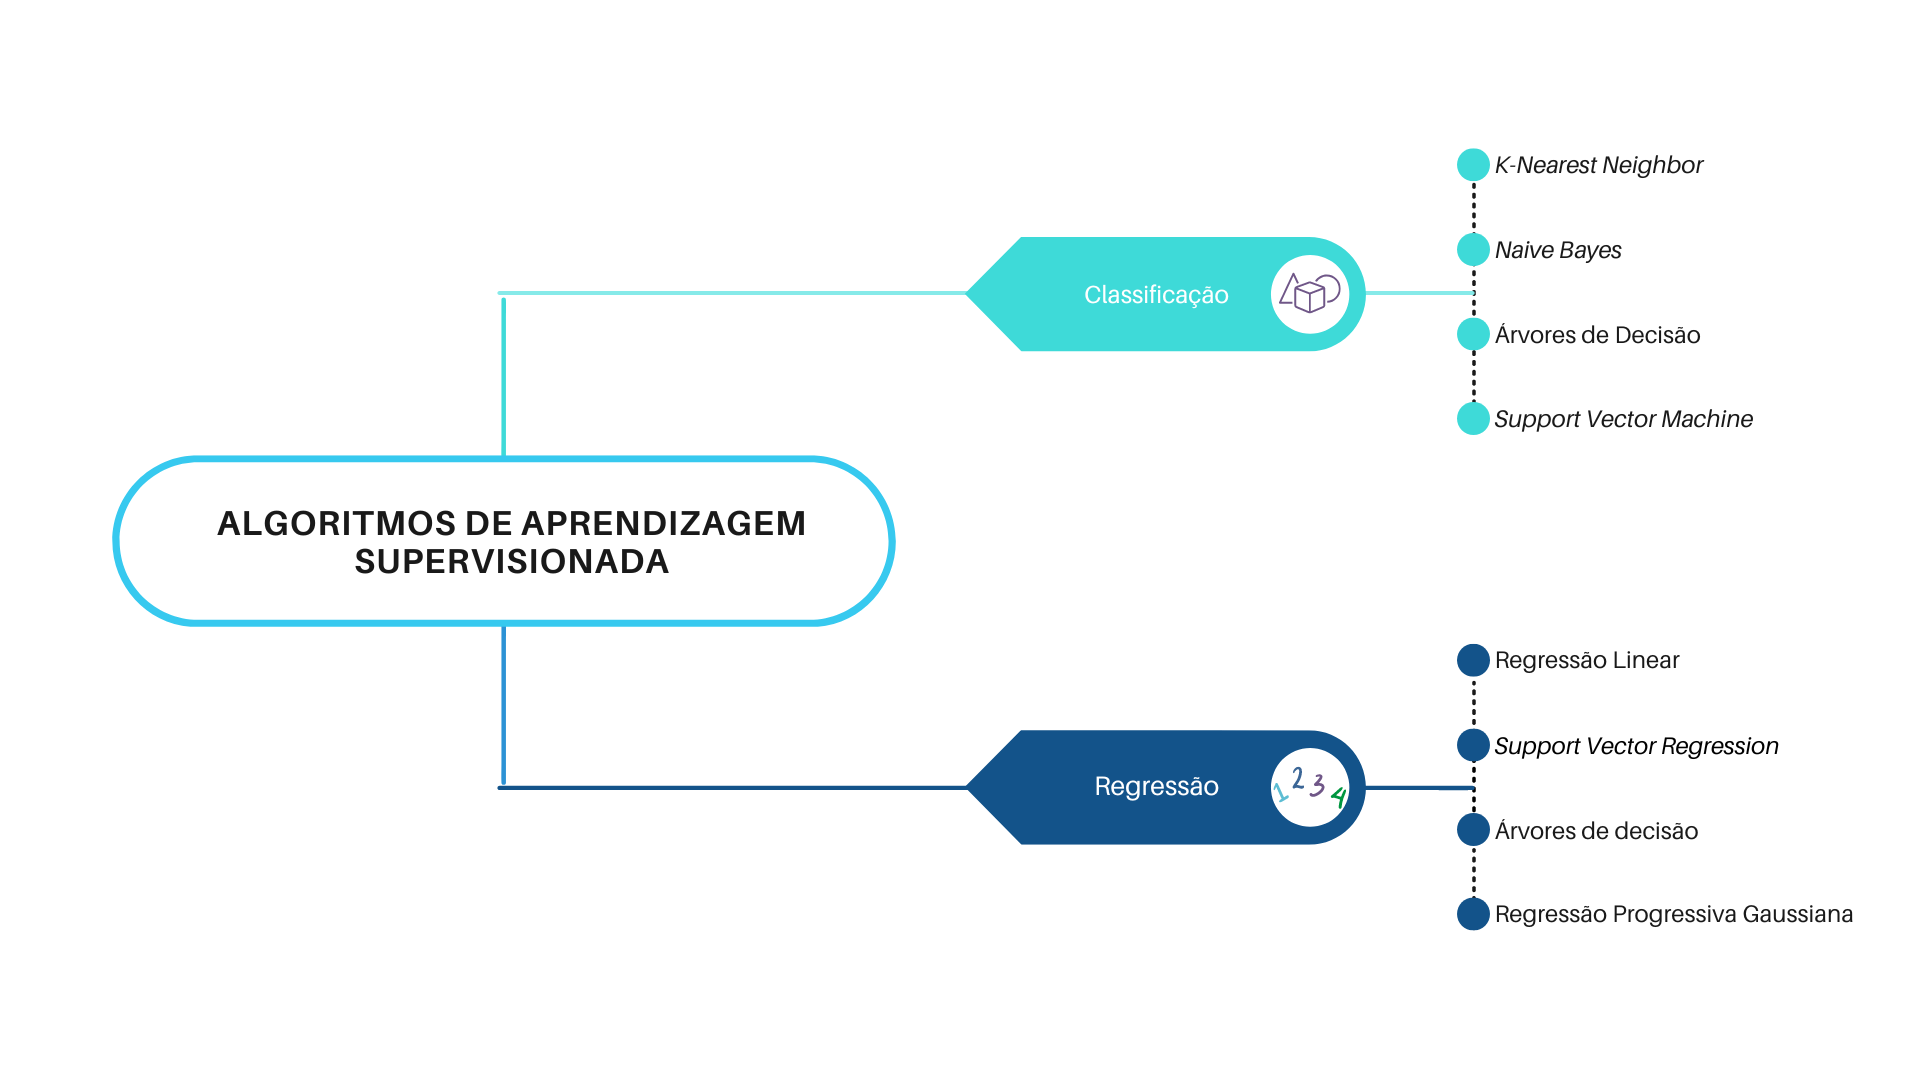
\includegraphics[width=0.9\linewidth]{fig/Capitulo2/3.png}
    \caption{Exemplos de algoritmos de aprendizagem supervisionada}
    \label{fig:enter-label3}
\end{figure}
 
 \subsection{Deep learning}

Os algoritmos deep learning fazem parte de um subconjunto dos algoritmos de machine learning. Eles se baseiam em redes neurais, onde conseguem através de várias camadas de neurônios uma aprendizagem profunda sem a intervenção humana, simulando um cérebro humano.

A vantagem da utilização da aprendizagem profunda é a identificações de padrões com um maior volume de dados, onde eles podem ser mais complexos e também não precisam ser estruturados, como por exemplo dados de imagem e voz.

Há 3 arquiteturas de redes neurais abordadas nesse trabalho, redes neurais recorrentes (RNN), memória de curto prazo longa (LSTM) e redes neurais convolucionais (CNN).

 \subsubsection{RNN - Recurrent Neural Network}

    Além dos dados da camada anterior, os neurônios da rede neural recorrente também recebem o resultado da operação matemática que eles mesmos realizaram no período temporal anterior. Dessa forma, as RNNs consideram uma dependência temporal entre os dados de entrada.

 \subsubsection{LSTM - Long Short Term Memory}
 
    As LSTMs são consideradas evoluções da RNNs, por resolver um problema comum nas redes neurais recorrentes, os gradientes que explodem ou desaparecem, que fazem com que a relação temporal que a rede deve aprender se perca com o tempo. Este esquecimento é resolvido pelos neurônios das redes LSTM que mantêm uma célula exclusiva para o armazenamento e fluxo da memória além de portões do tipo entrada (\textit{input gate}), saída (\textit{output gate}) e esquecimento (\textit{forget gate}), que controlam esse fluxo.

    \begin{figure}[!htp]
        \centering
        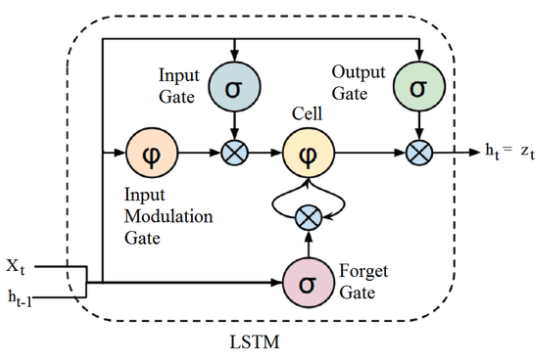
\includegraphics[width=.8\linewidth]{fig/Capitulo2/ArquiteturaLSTM.png}
        \caption{Arquitetura do modelo LSTM}
        \label{fig:enter-labelLSTM}
    \end{figure}

    Na estrutura apresentada na Figura \ref{fig:enter-labelLSTM}, retirada do site \cite{DeepLearning}, o \textit{input modulation gate} atua como um ponto chave. Ele recebe tanto as informações $X_t$ quanto $h_{t-1}$, desempenhando uma função de regulação que filtra os valores a serem retidos, de maneira similar ao processo do portão de esquecimento. Enquanto este último remove dados irrelevantes da célula, o portão de entrada acrescenta informações essenciais. Por sua vez, o portão de saída extrai dados pertinentes para a saída. Essas portas desempenham um papel crucial na regulação dos dados, empregando funções de ativação e matrizes de peso.

 \subsubsection{CNN - Convolutional Neural Network}
    Utiliza aprendizagem supervisionada. Nas camadas de convolução, os filtros são aplicados para destacar padrões locais nos dados e reduzir sua dimensão. Os resultados dos filtros são combinados por operações de pooling. Nas camadas mais profundas, espera-se que os dados de menor dimensão ainda contenham informações relevantes sobre os padrões locais. Em seguida, os dados passam por uma estrutura de FFN (Feedforward Neural Network) para realizar a tarefa de classificação.

\begin{table}[!ht]
    \centering
    \begin{tabular}{|c|c|c|}
    \hline
        Arquiteturas & Natureza dos Dados & Tarefas Realizadas \\
    \hline
        RNN & \makecell{Adequadas para processar dados \\ sequenciais, como sequências \\ de texto.} & \makecell{Tradução automática, análise de \\ sentimentos, classificação de textos.} \\
    \hline
        LSTM & \makecell{As LSTMs são uma variação das \\ RNNs projetadas para lidar com \\ sequências de dados de série \\ temporal, como dados climáticos, \\ dados financeiros  ou registros \\ de atividades} & \makecell{Tradução automática, análise de \\ sentimentos, classificação de textos \\ e modelar dependências de longo \\ prazo em sequências de dados \\ de séries temporais.}\\
        
    \hline
        CNN & \makecell{Amplamente utilizadas em tarefas \\ de visão computacional, onde os \\ dados de entrada são \\ imagens representadas em formato \\ de grade bidimensional.} & \makecell{Classificação de imagens e detecção \\ de objetos.} \\
    \hline
    \end{tabular}
    \caption{RNNs, LSTMs e CNNs}
    \label{tab:my_label21}
\end{table}

%\section{Ciência de dados para o bem}
\newpage
\section{COVID-19 no centro-oeste brasileiro: um estudo de caso de ciência de dados}

Nesta seção, apresenta-se avaliações exploratórias dos dados coletados a partir das fontes \textit{OpenDatasus} e Coronavírus Brasil. As Figuras \ref{fig:my_label1}, \ref{fig:my_label5}, \ref{fig:my_label9} e \ref{fig:my_label13} exibem as quantidades de vacinas aplicadas por Estado durante o período de Janeiro de 2021 a Junho de 2022, incluindo a soma de todas as doses administradas. Enquanto as Figuras \ref{fig:my_label2}, \ref{fig:my_label6}, \ref{fig:my_label10} e \ref{fig:my_label14} proporcionam uma diferenciação dessas quantidades, especificamente pelas doses administradas no mesmo intervalo temporal conforme mencionado anteriormente.

Ao analisar esses gráficos, podemos concluir que a maioria das vacinas foi administrada no segundo semestre de 2021, evidenciando picos de vacinação nesse período para os quatro cenários abordados.

Esses gráficos permitem afirmar que, nos três Estados avaliados e no Distrito Federal, a grande maioria da população recebeu apenas até a segunda dose da vacina. Ao comparar com as doses adicionais e de reforço, a discrepância é notável, destacada nos dois primeiros gráficos de cada Estado e do Distrito Federal.

Por fim, ao compararmos os gráficos de vacinação com os de óbitos, \ref{fig:my_label4}, \ref{fig:my_label8}, \ref{fig:my_label12} e \ref{fig:my_label16}, podemos constatar que, após o pico de vacinação no segundo semestre de 2021, houve uma queda significativa no número de óbitos, uma tendência que se manteve até o primeiro semestre de 2022. O código fonte está disponível no Github\cite{Github}.
\newpage


\begin{center}
    \textbf{Estado de Goiás}
\end{center}

    \begin{figure}[!htp]
        \centering
        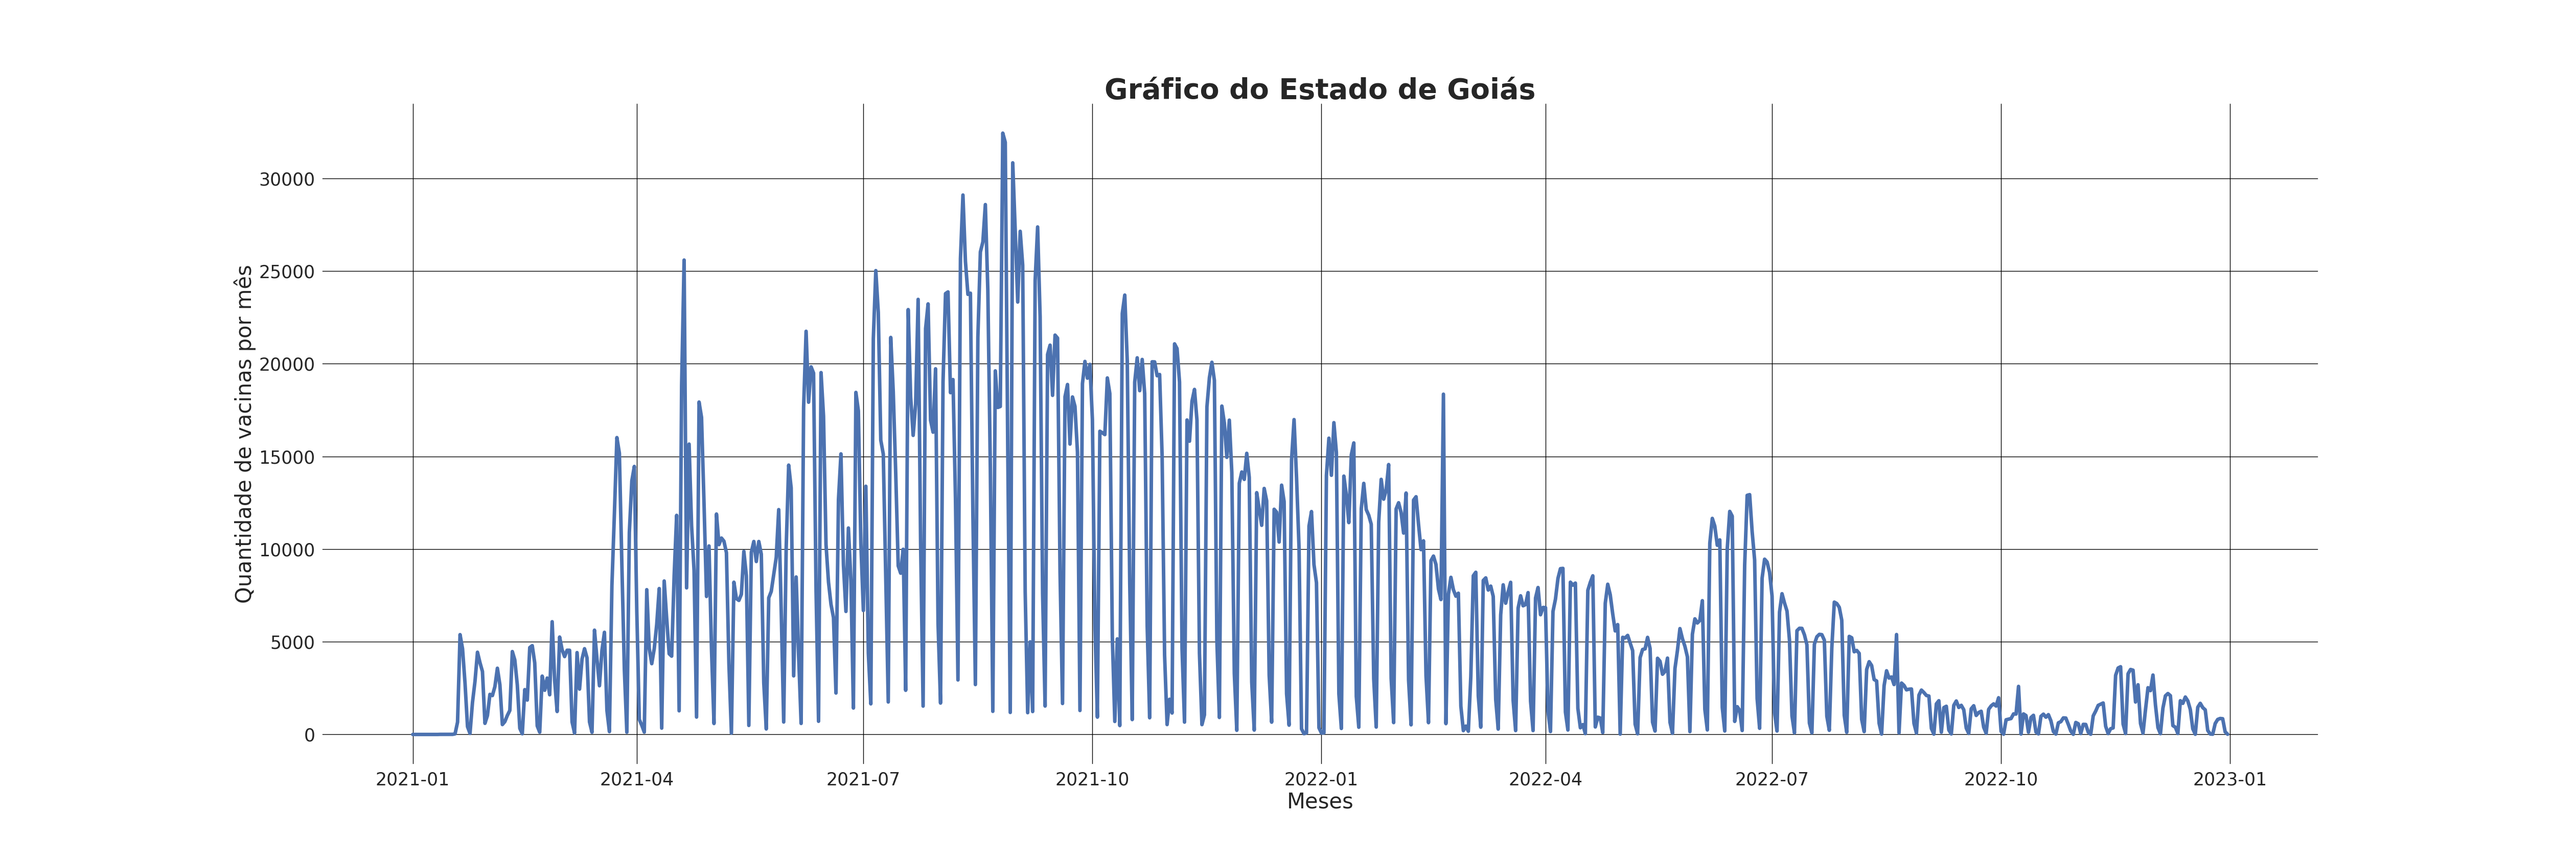
\includegraphics[width=.99\linewidth]{fig/Vacinação/2-Goias.png}
        \caption{Quantidade de vacinas aplicadas por mês no Estado de Goiás.}
        \label{fig:my_label1}
    \end{figure}
    
    \begin{figure}[!htp]
        \centering
        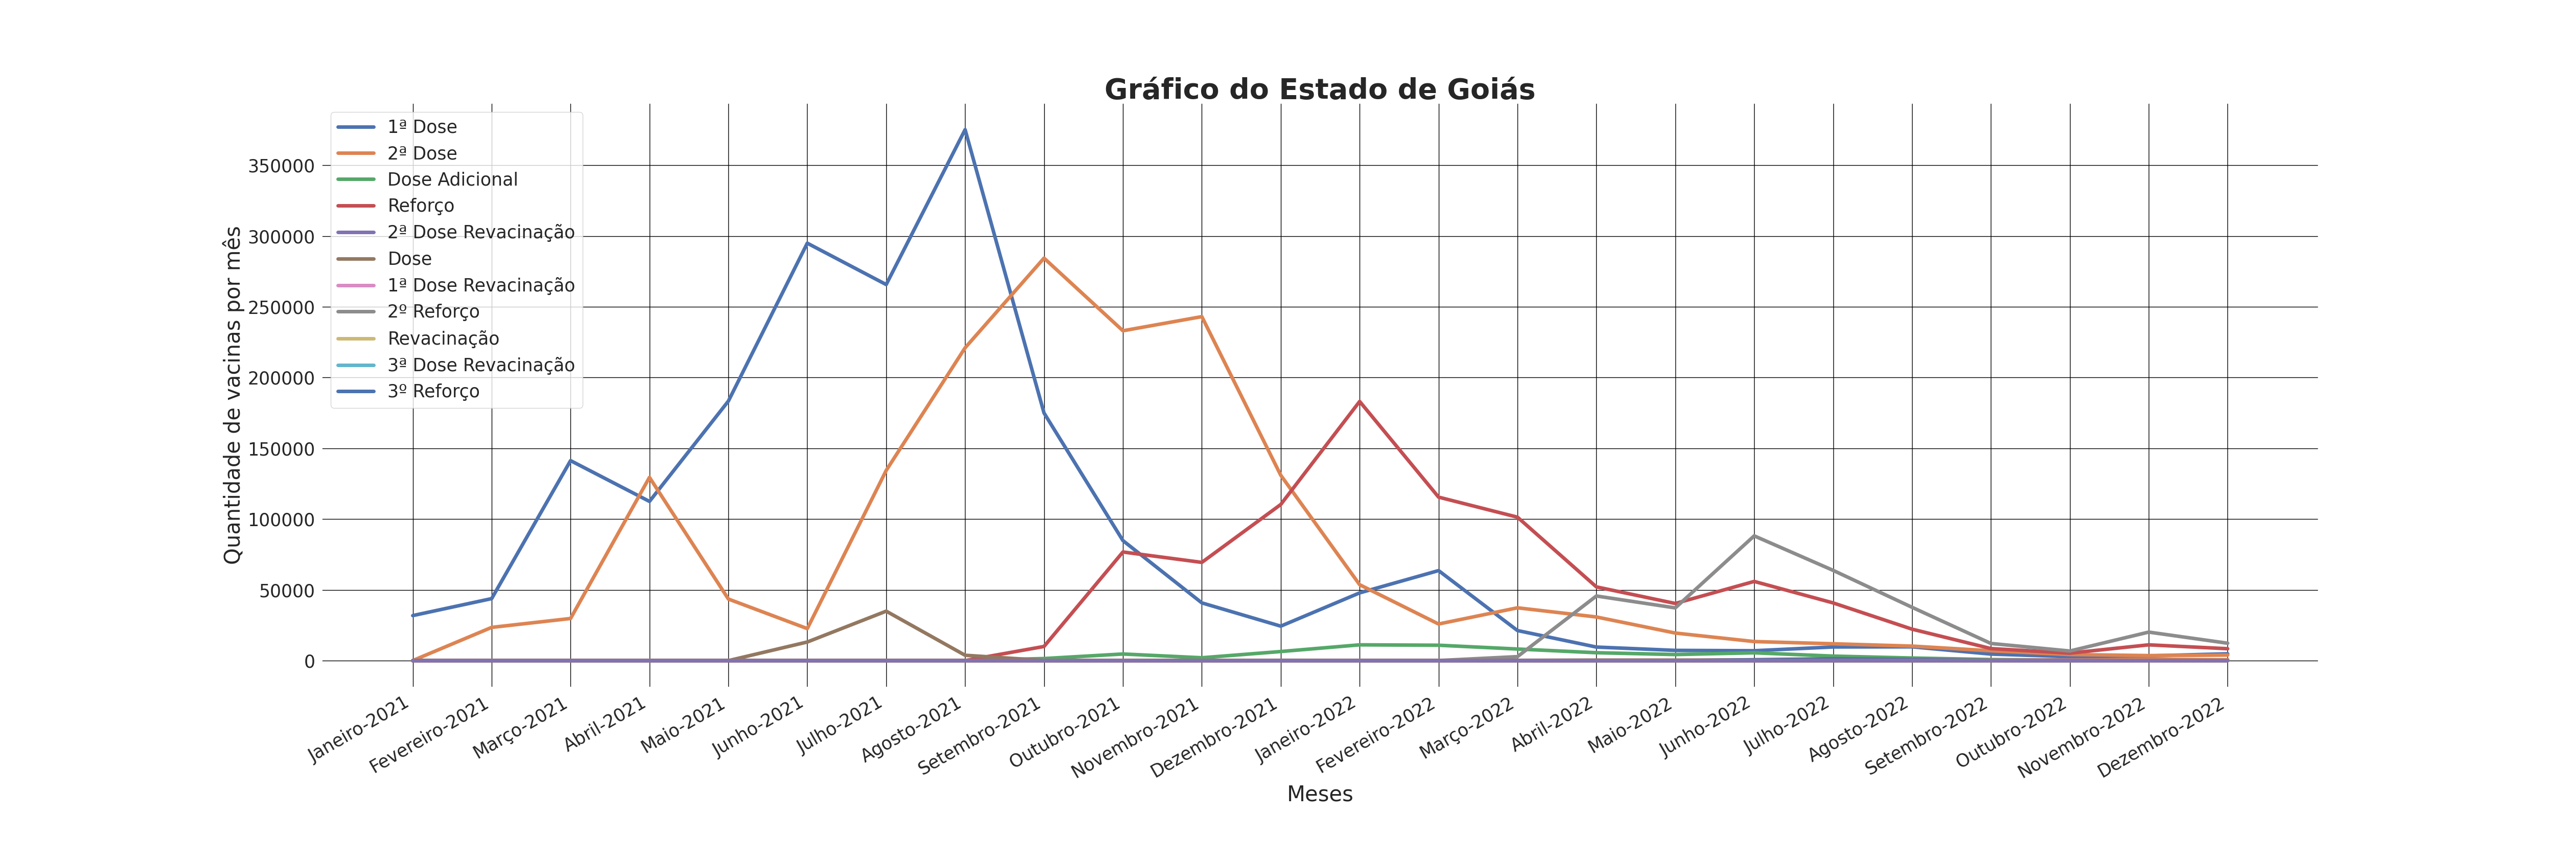
\includegraphics[width=.99\linewidth]{fig/Vacinação/1-Goias.png}
        \caption{Quantidade de vacinas aplicadas por tipo de dose desde o início da vacinação naquele Estado até junho de 2022 no Estado de Goiás.}
        \label{fig:my_label2}
    \end{figure}

    % \begin{figure}[!htp]
    %     \centering
    %     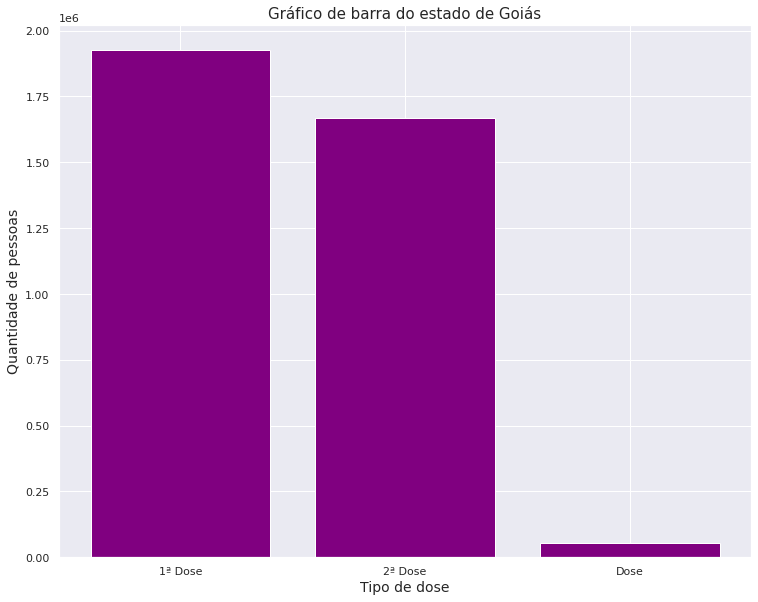
\includegraphics[width=.99\linewidth]{fig/Vacinação/3-Goias.png}
    %     \caption{Quantidade de pessoas vacinadas na primeira, segunda e dose única no Estado de Goiás.}
    %     \label{fig:my_label3}
    % \end{figure}
    
    % \begin{figure}[htp]
    %     \centering
    %     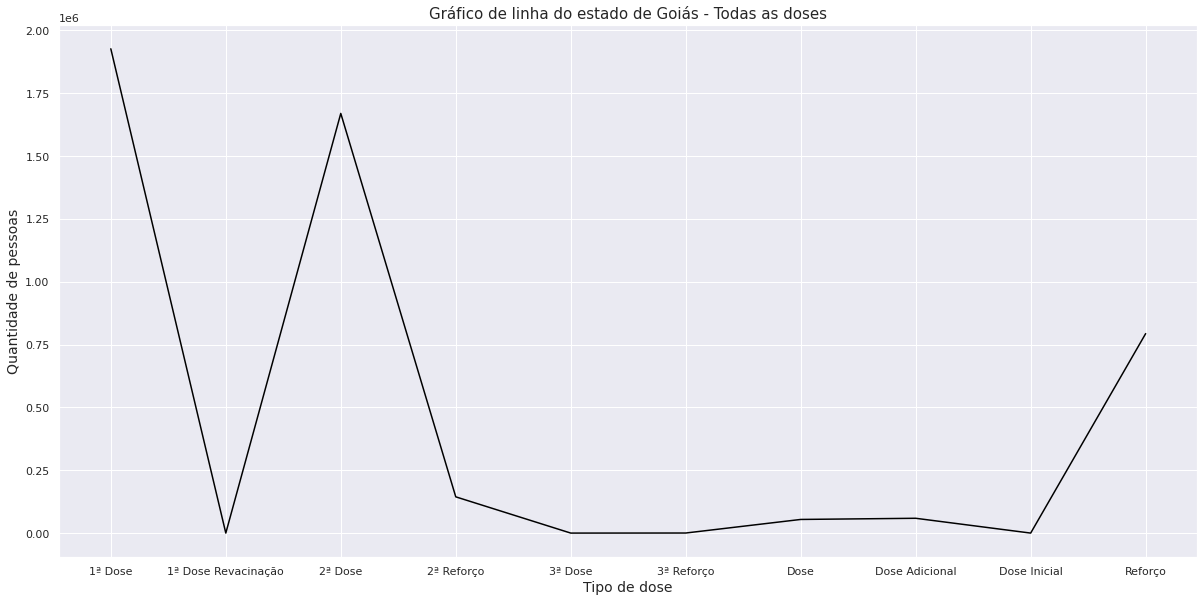
\includegraphics[width=.99\linewidth]{fig/Vacinação/4-Goias.png}
    %     \caption{Quantidade de pessoas vacinadas em todas as doses no Estado de Goiás.}
    %     \label{fig:my_label4}
    % \end{figure}


    \begin{figure}[!htp]
        \centering
        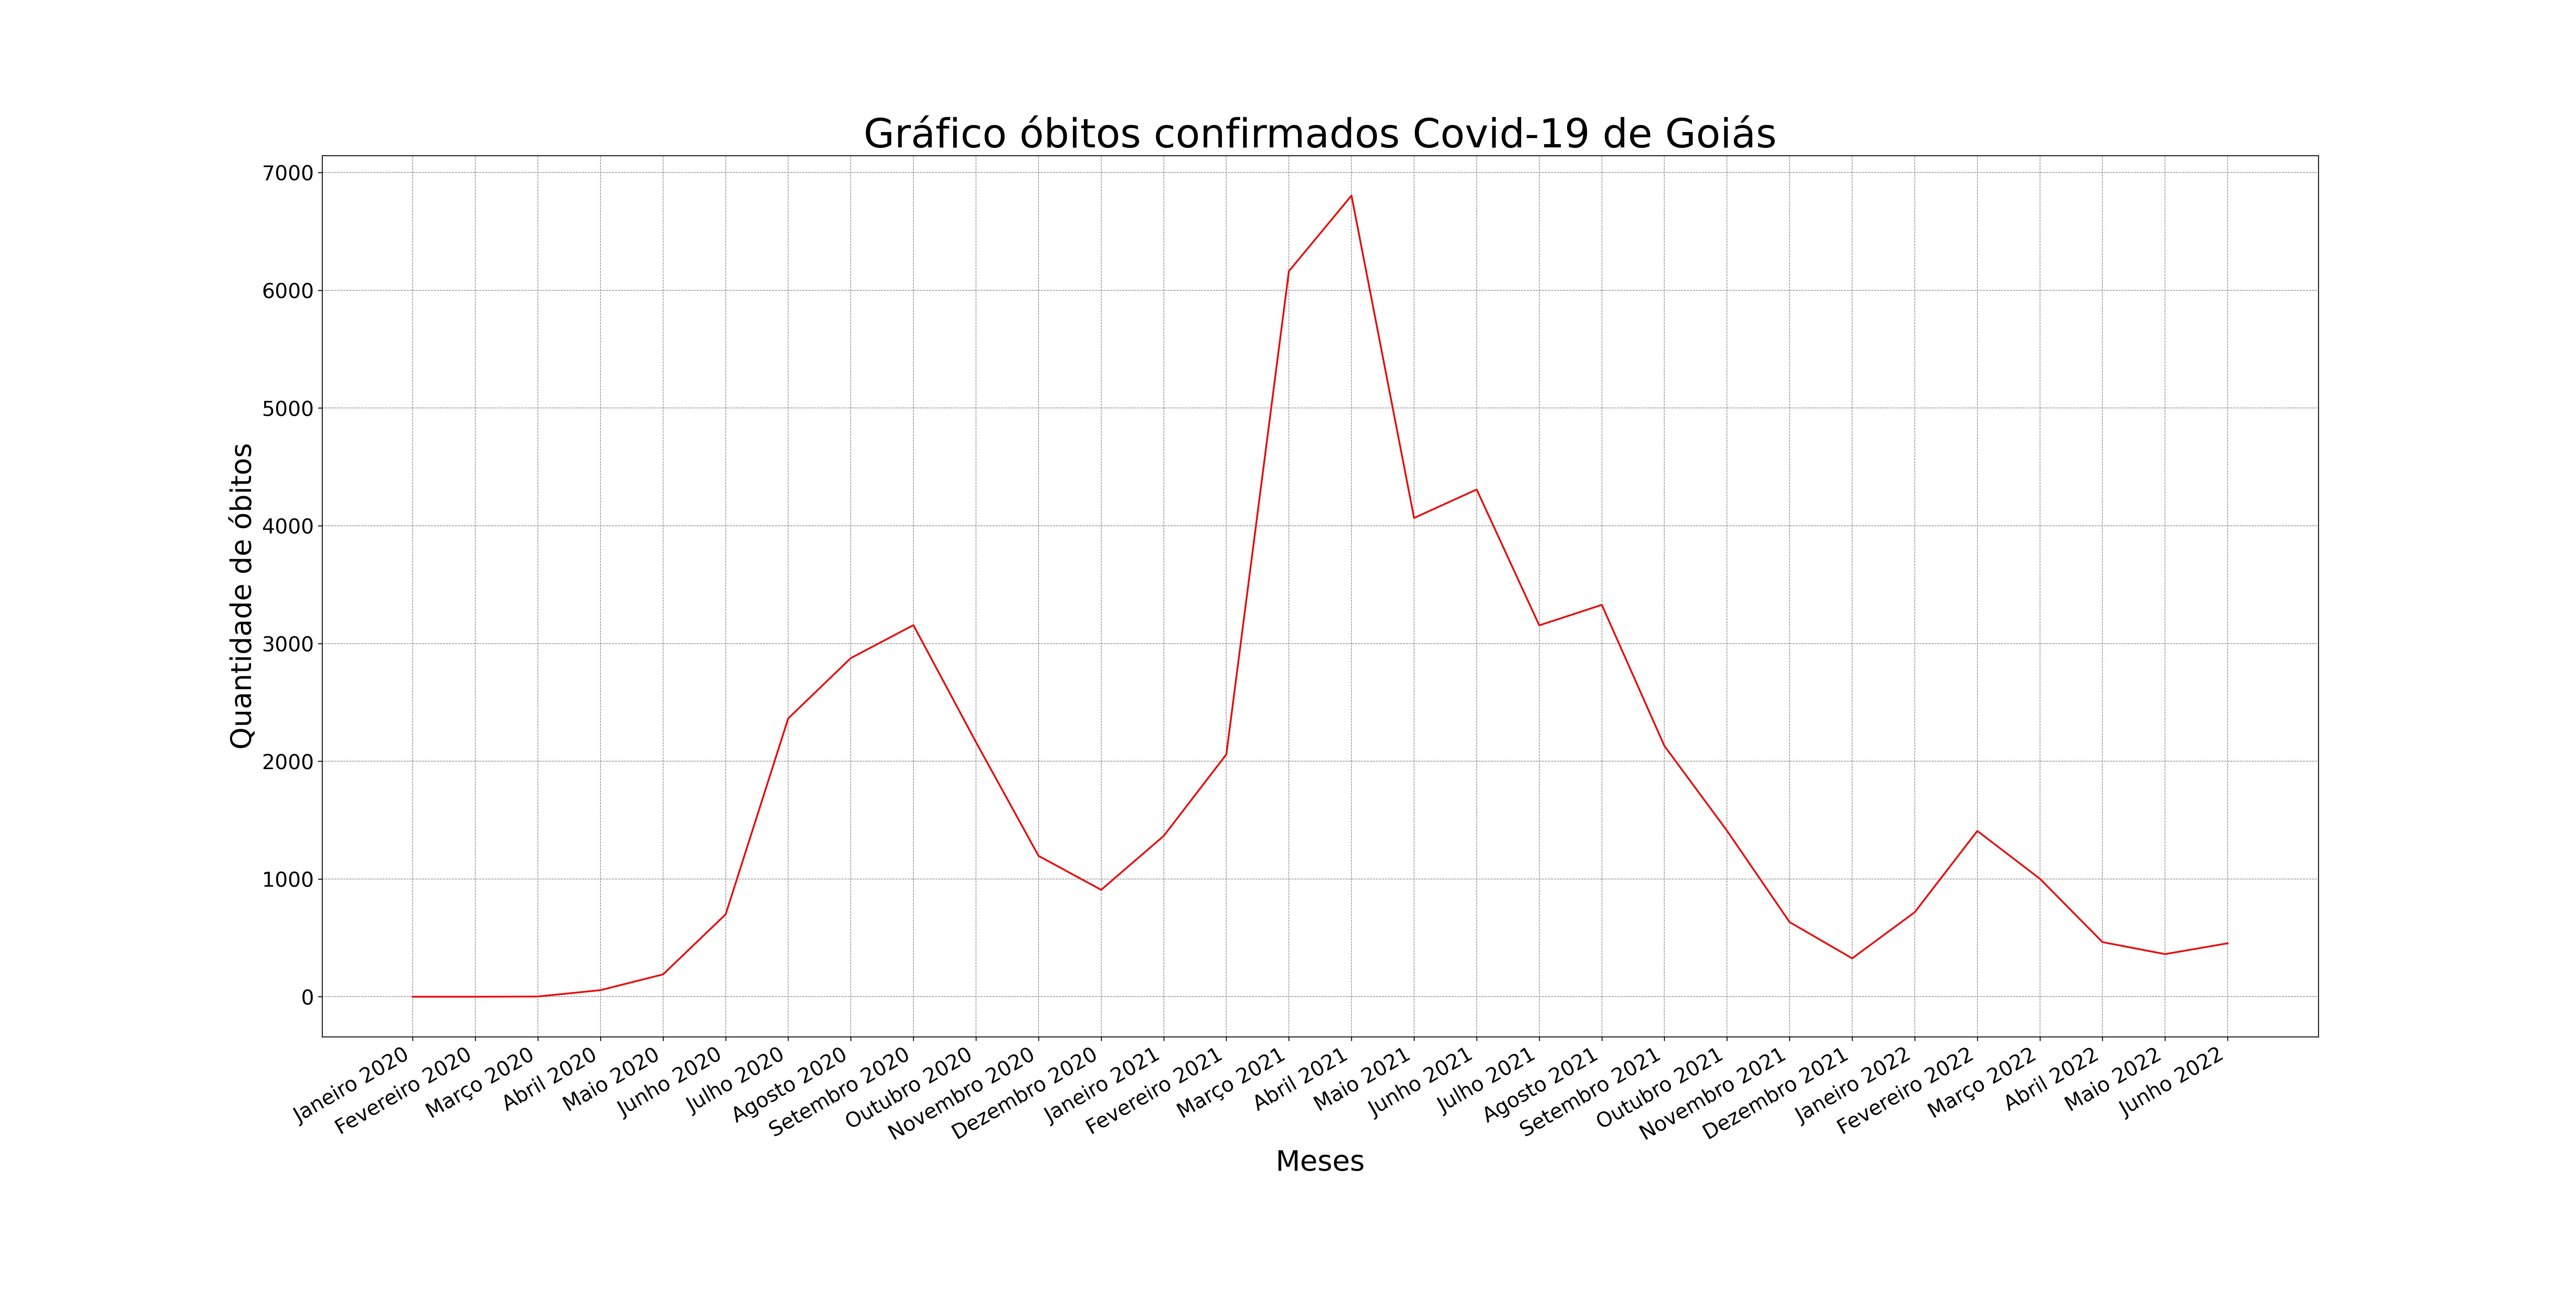
\includegraphics[width=.99\linewidth]{fig/Obitos/GO_Obitos.png}
        \caption{Quantidade de óbitos mensal no Estado de Goiás.}
        \label{fig:my_label4}
    \end{figure}


\begin{center}
    \textbf{Estado de Mato Grosso}
\end{center}

    \begin{figure}[!htp]
        \centering
        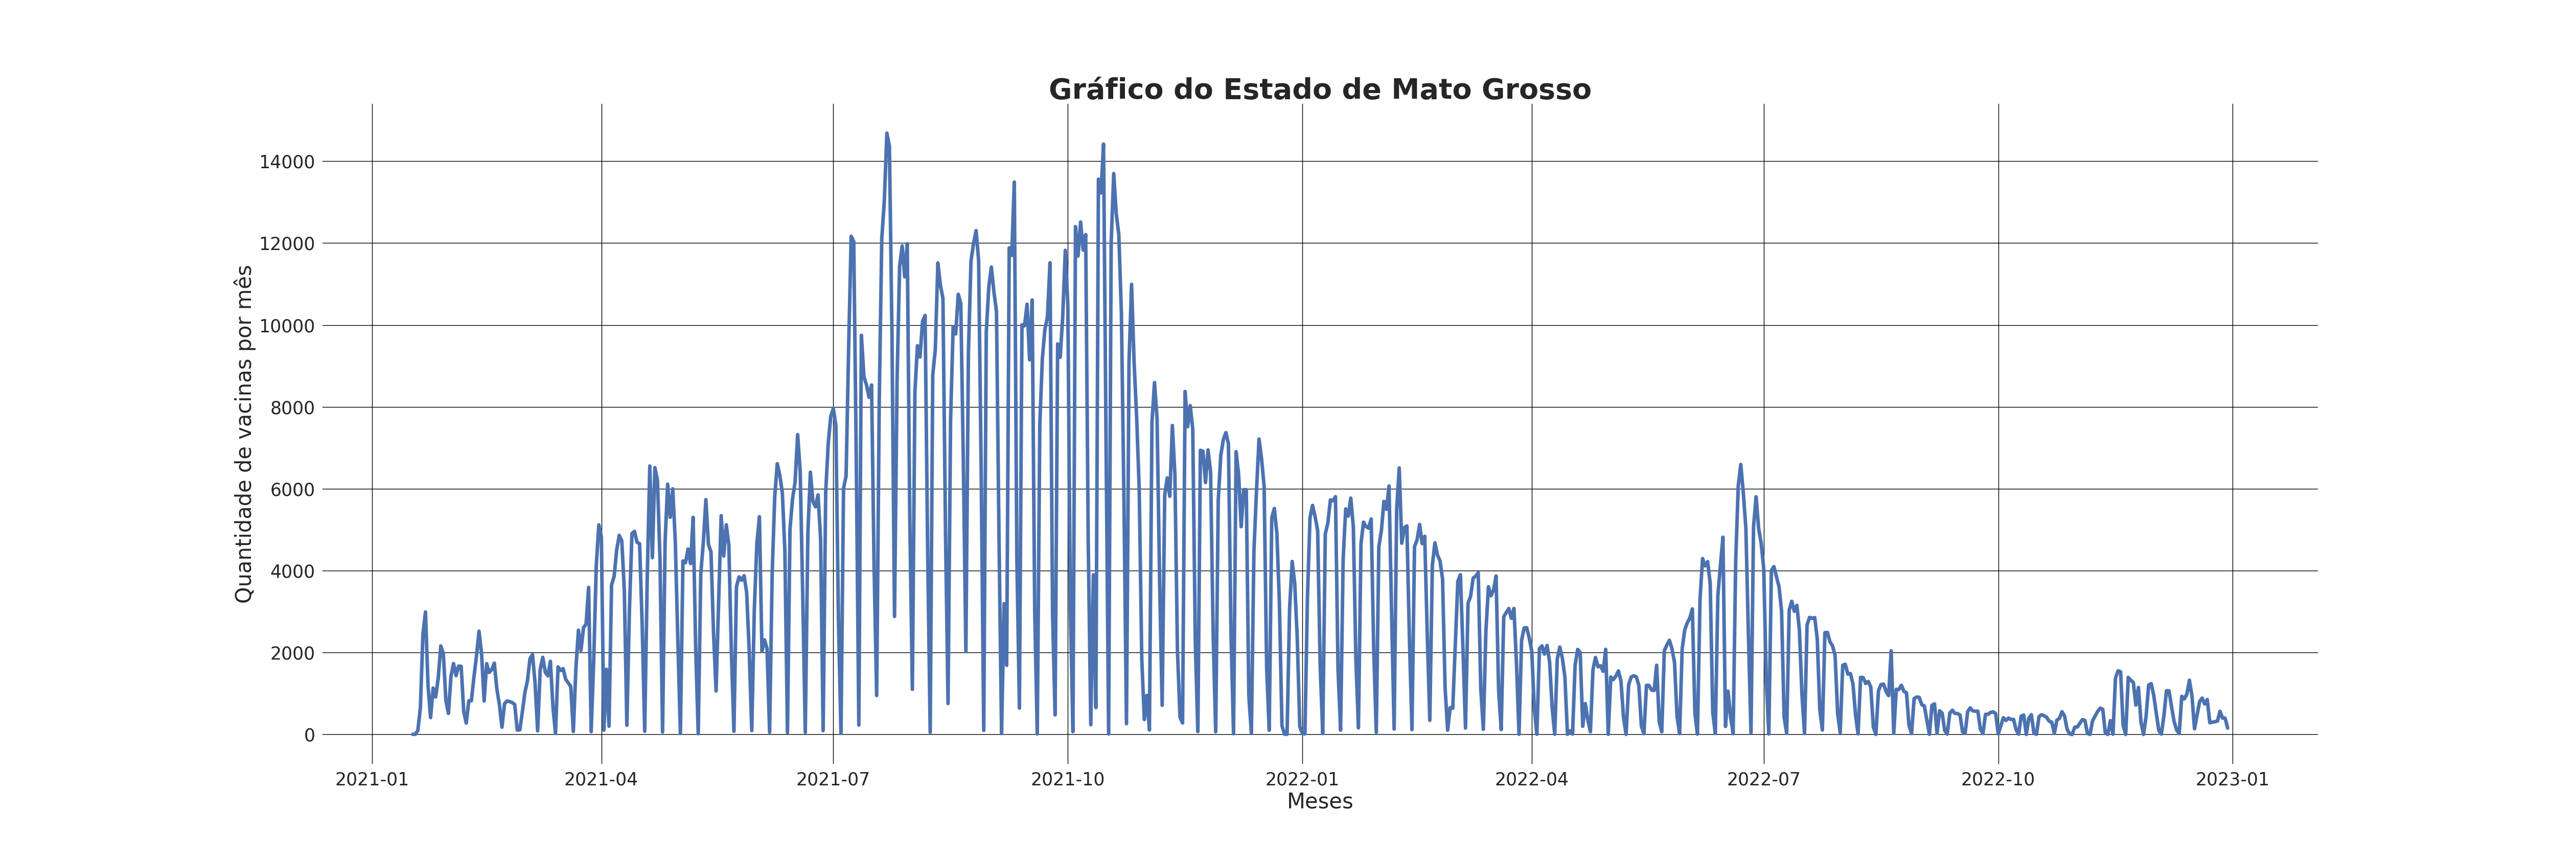
\includegraphics[width=.99\linewidth]{fig/Vacinação/2-MatoGrosso.png}
        \caption{Quantidade de vacinas aplicadas por mês no Estado de Mato Grosso.}
        \label{fig:my_label5}
    \end{figure}
    
    \begin{figure}[!htp]
        \centering
        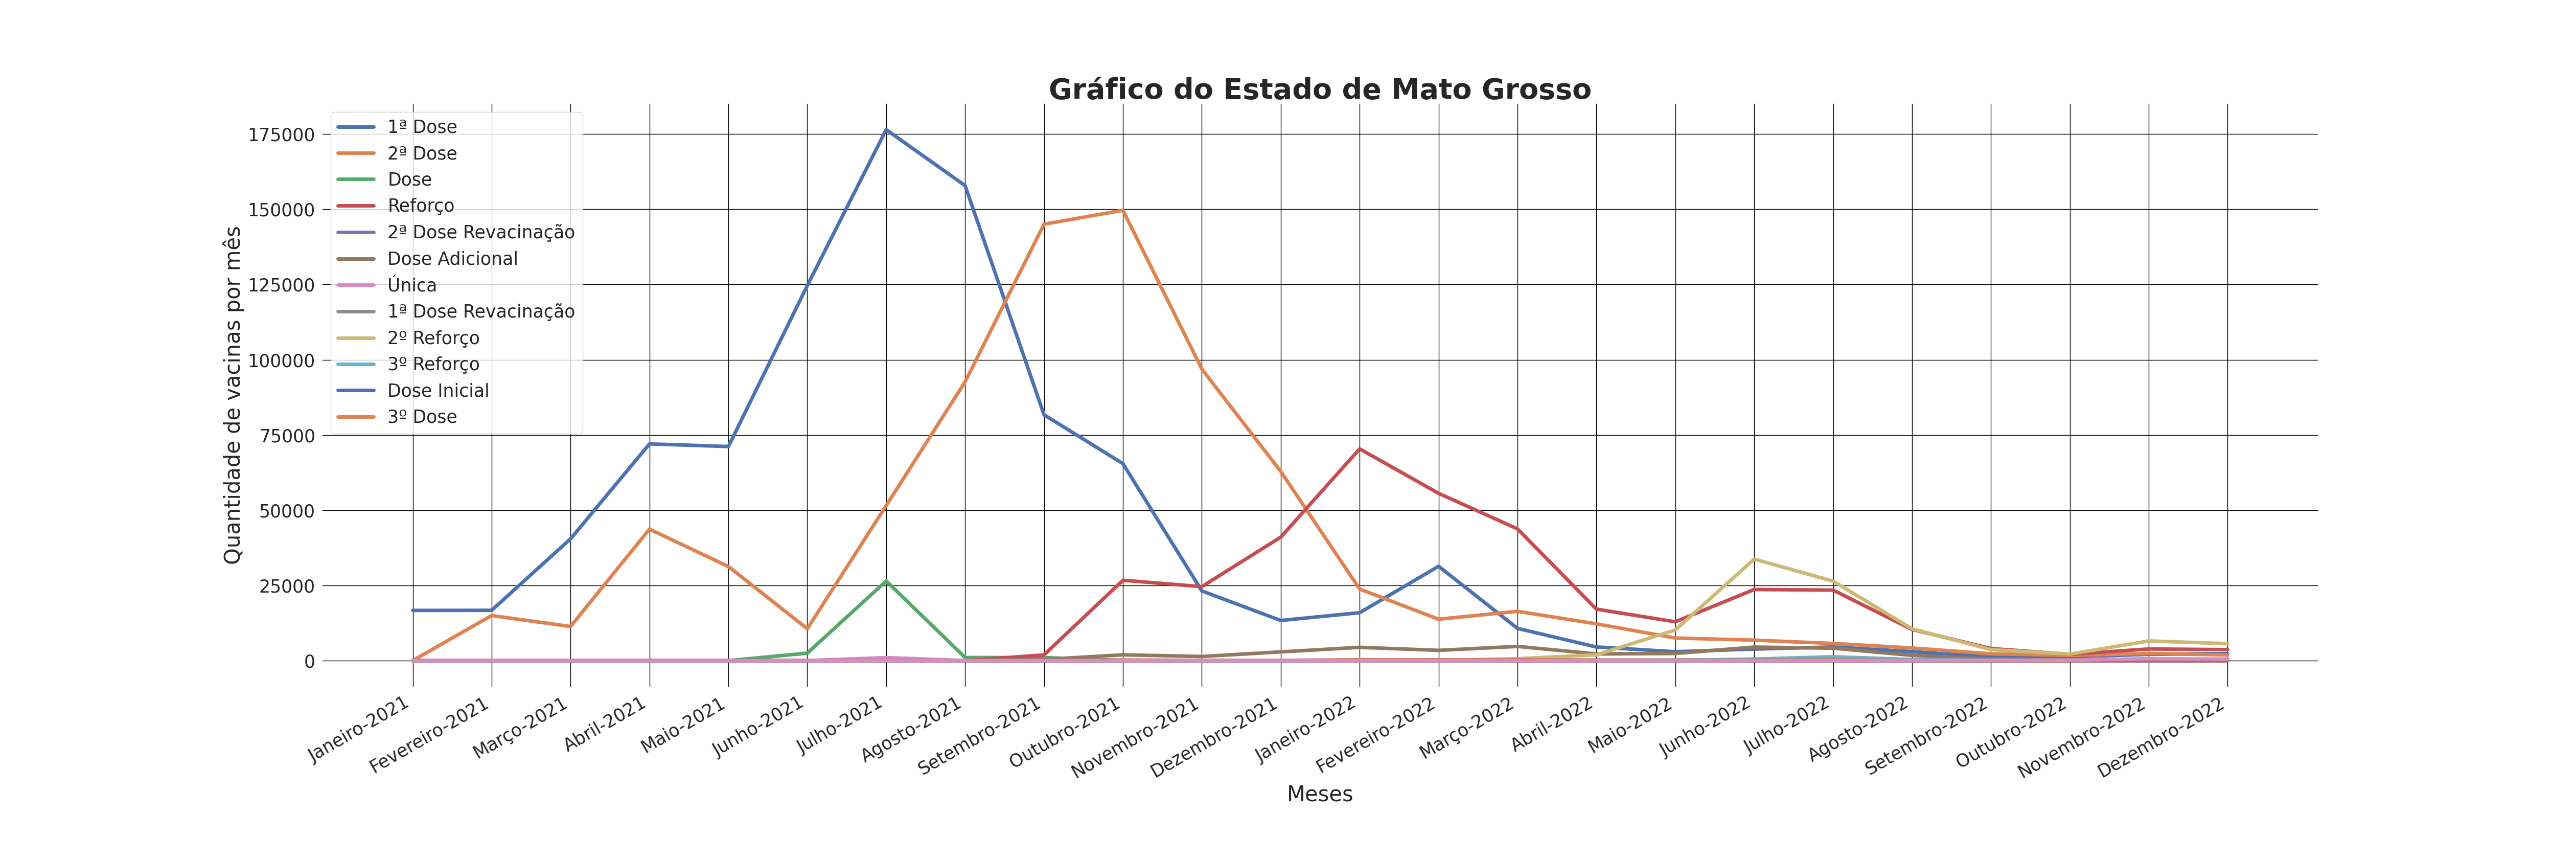
\includegraphics[width=.99\linewidth]{fig/Vacinação/1-MatoGrosso.png}
        \caption{Quantidade de vacinas aplicadas por tipo de dose desde o início da vacinação naquele Estado até junho de 2022 no Estado de Mato Grosso.}
        \label{fig:my_label6}
    \end{figure}

    % \begin{figure}[!htp]
    %     \centering
    %     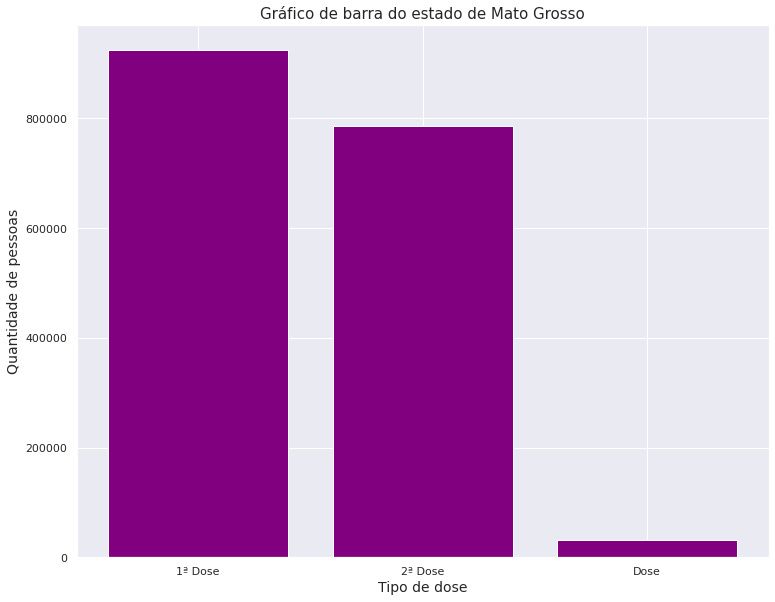
\includegraphics[width=.99\linewidth]{fig/Vacinação/3-MatoGrosso.png}
    %     \caption{Quantidade de pessoas vacinadas na primeira, segunda e dose única no Estado de Mato Grosso.}
    %     \label{fig:my_label7}
    % \end{figure}
    
    % \begin{figure}[htp]
    %     \centering
    %     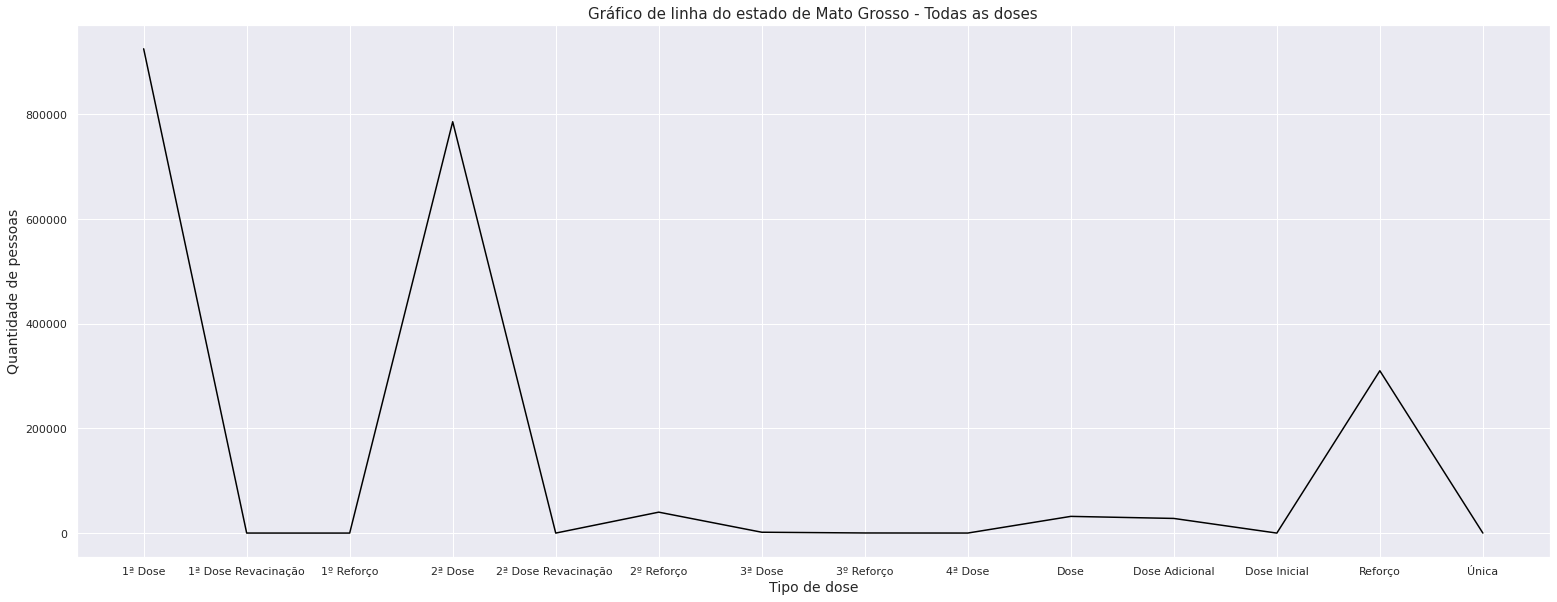
\includegraphics[width=.99\linewidth]{fig/Vacinação/4-MatoGrosso.png}
    %     \caption{Quantidade de pessoas vacinadas em todas as doses no Estado de Mato Grosso.}
    %     \label{fig:my_label8}
    % \end{figure}

    \begin{figure}[!htp]
        \centering
        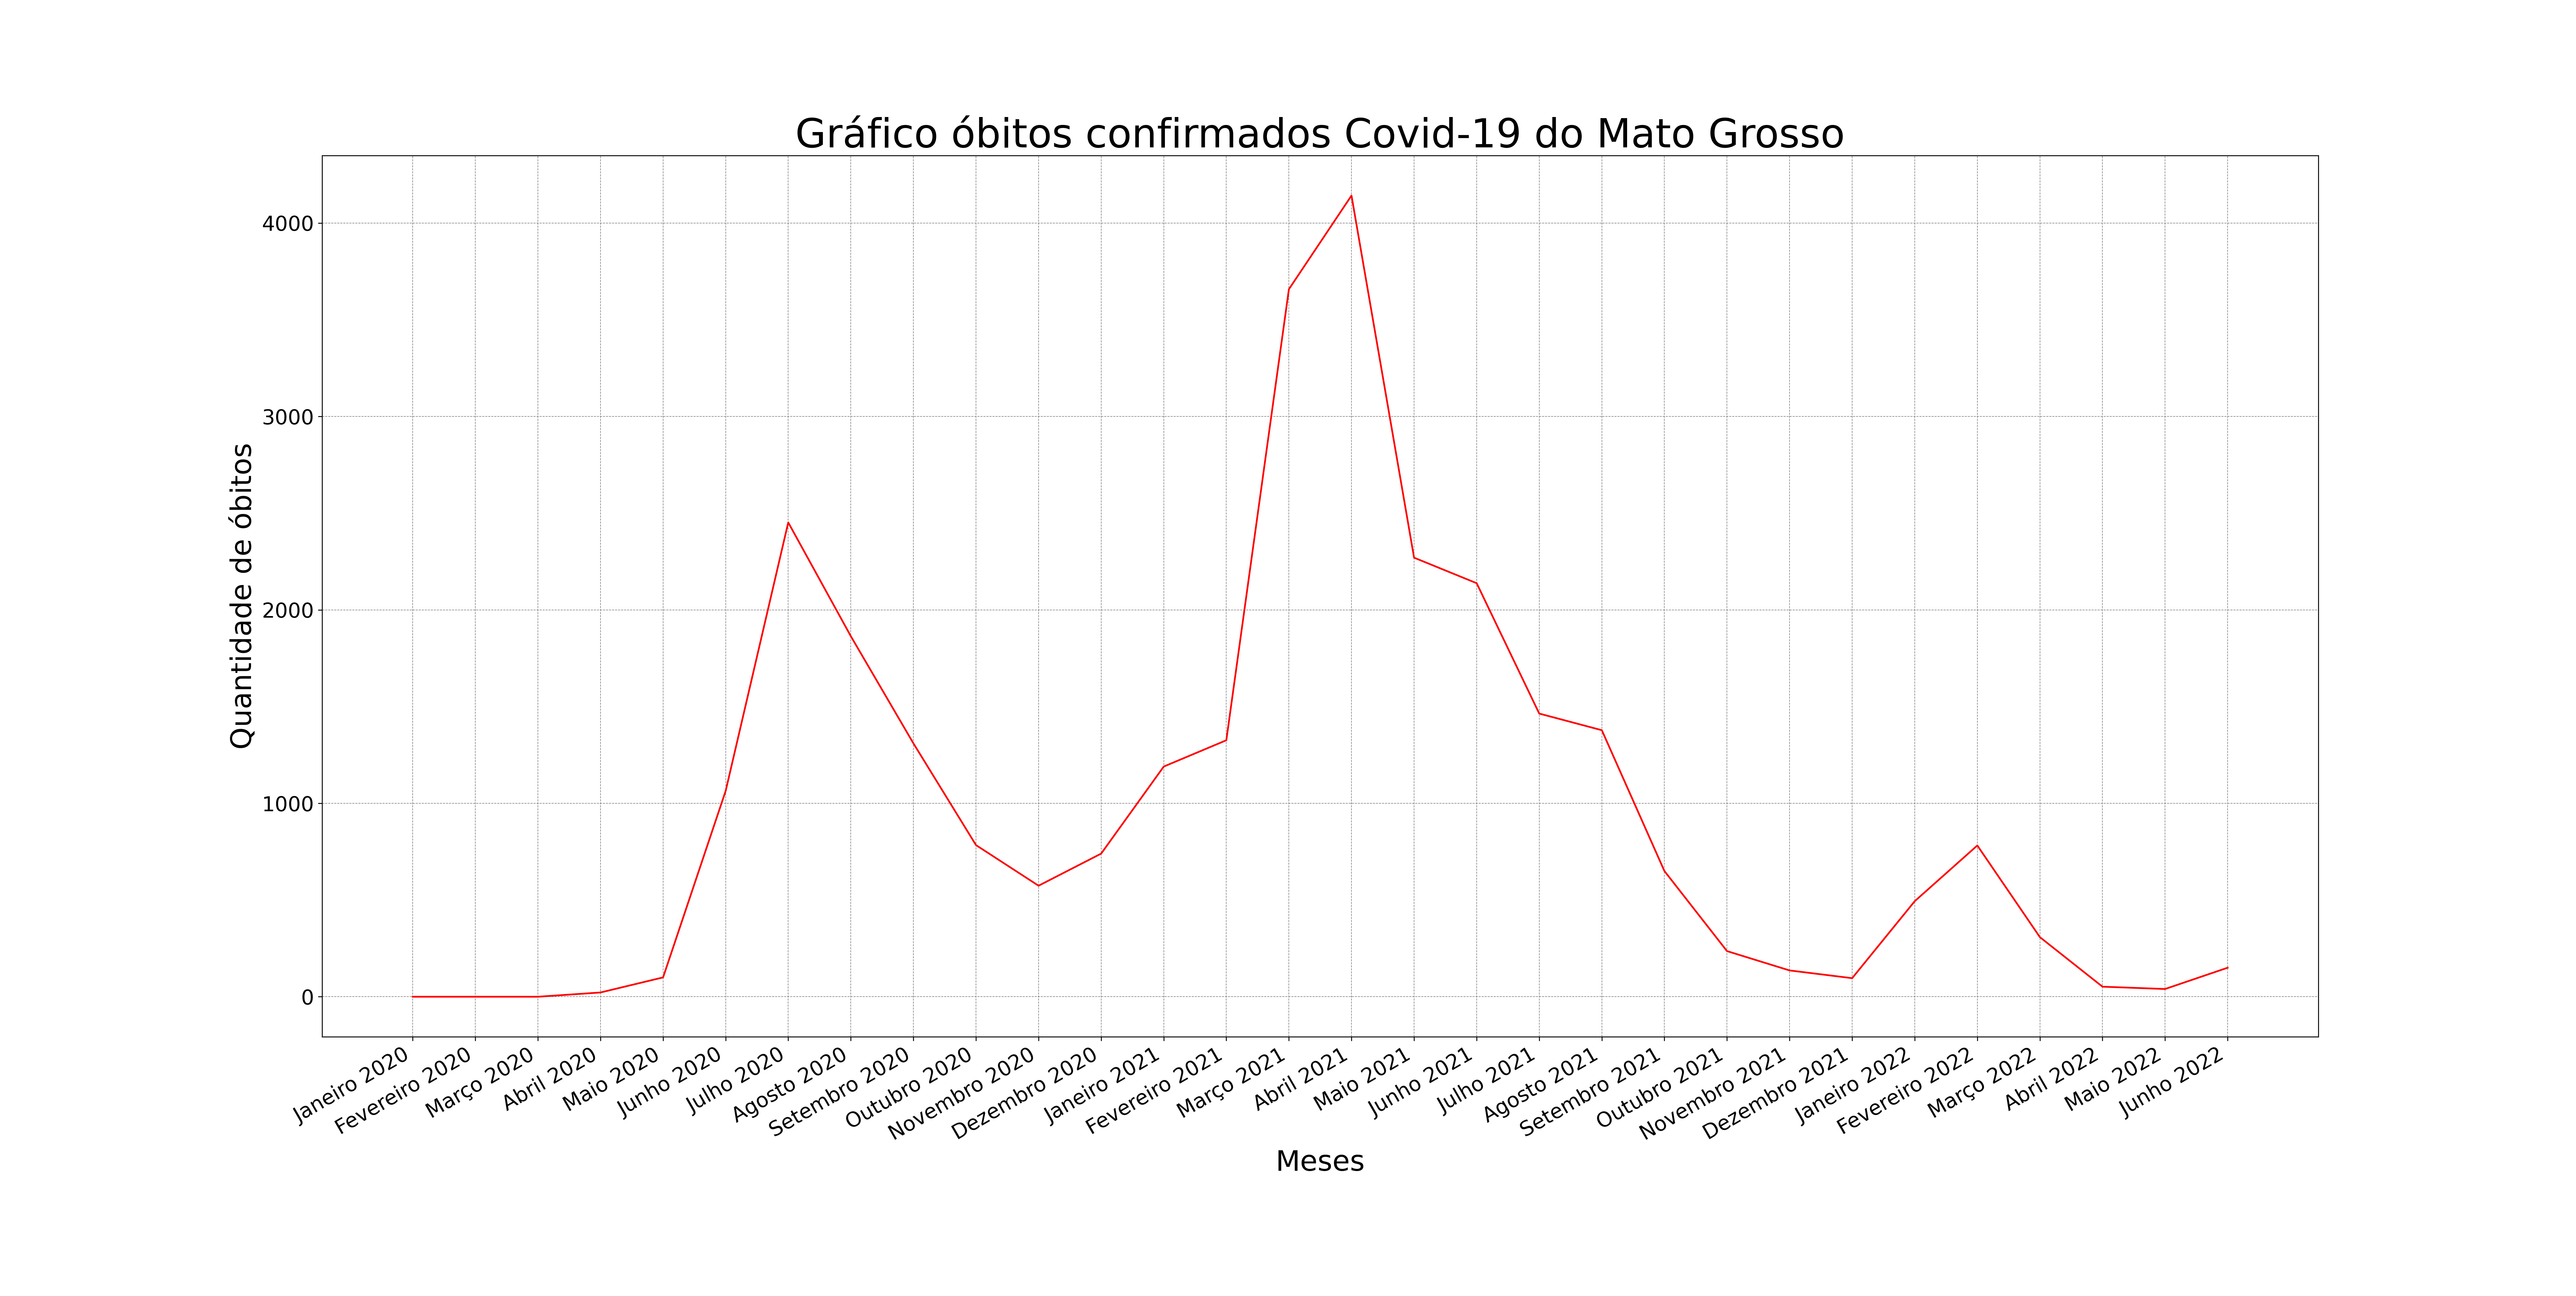
\includegraphics[width=.99\linewidth]{fig/Obitos/MT_Obitos.png}
        \caption{Quantidade de óbitos mensal no Estado de Mato Grosso.}
        \label{fig:my_label8}
    \end{figure}

\newpage
\begin{center}
    \textbf{Estado de Mato Grosso do Sul}
\end{center}

    \begin{figure}[!htp]
        \centering
        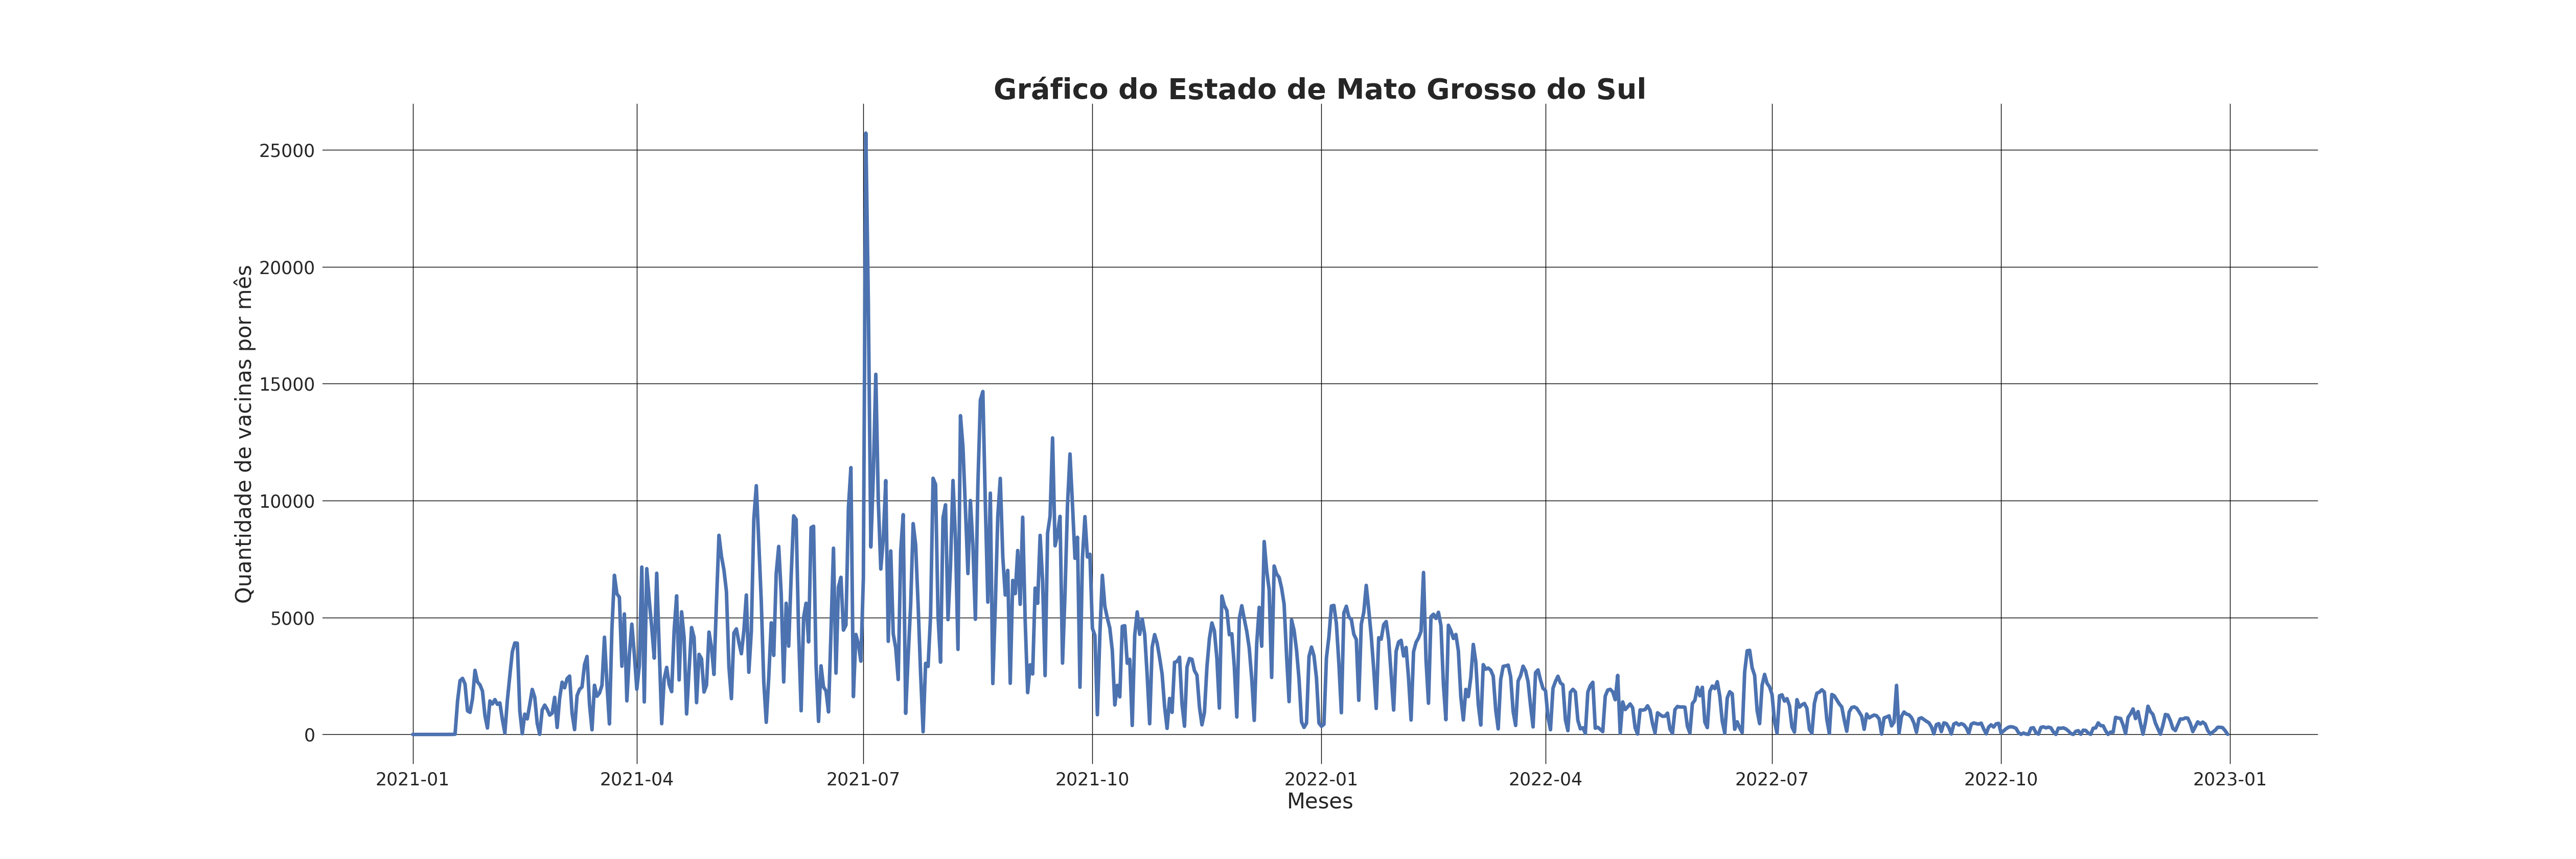
\includegraphics[width=.99\linewidth]{fig/Vacinação/1-MatoGrossodoSul.png}
        \caption{Quantidade de vacinas aplicadas por mês no Estado de Mato Grosso do Sul.}
        \label{fig:my_label9}
    \end{figure}
    
    \begin{figure}[!htp]
        \centering
        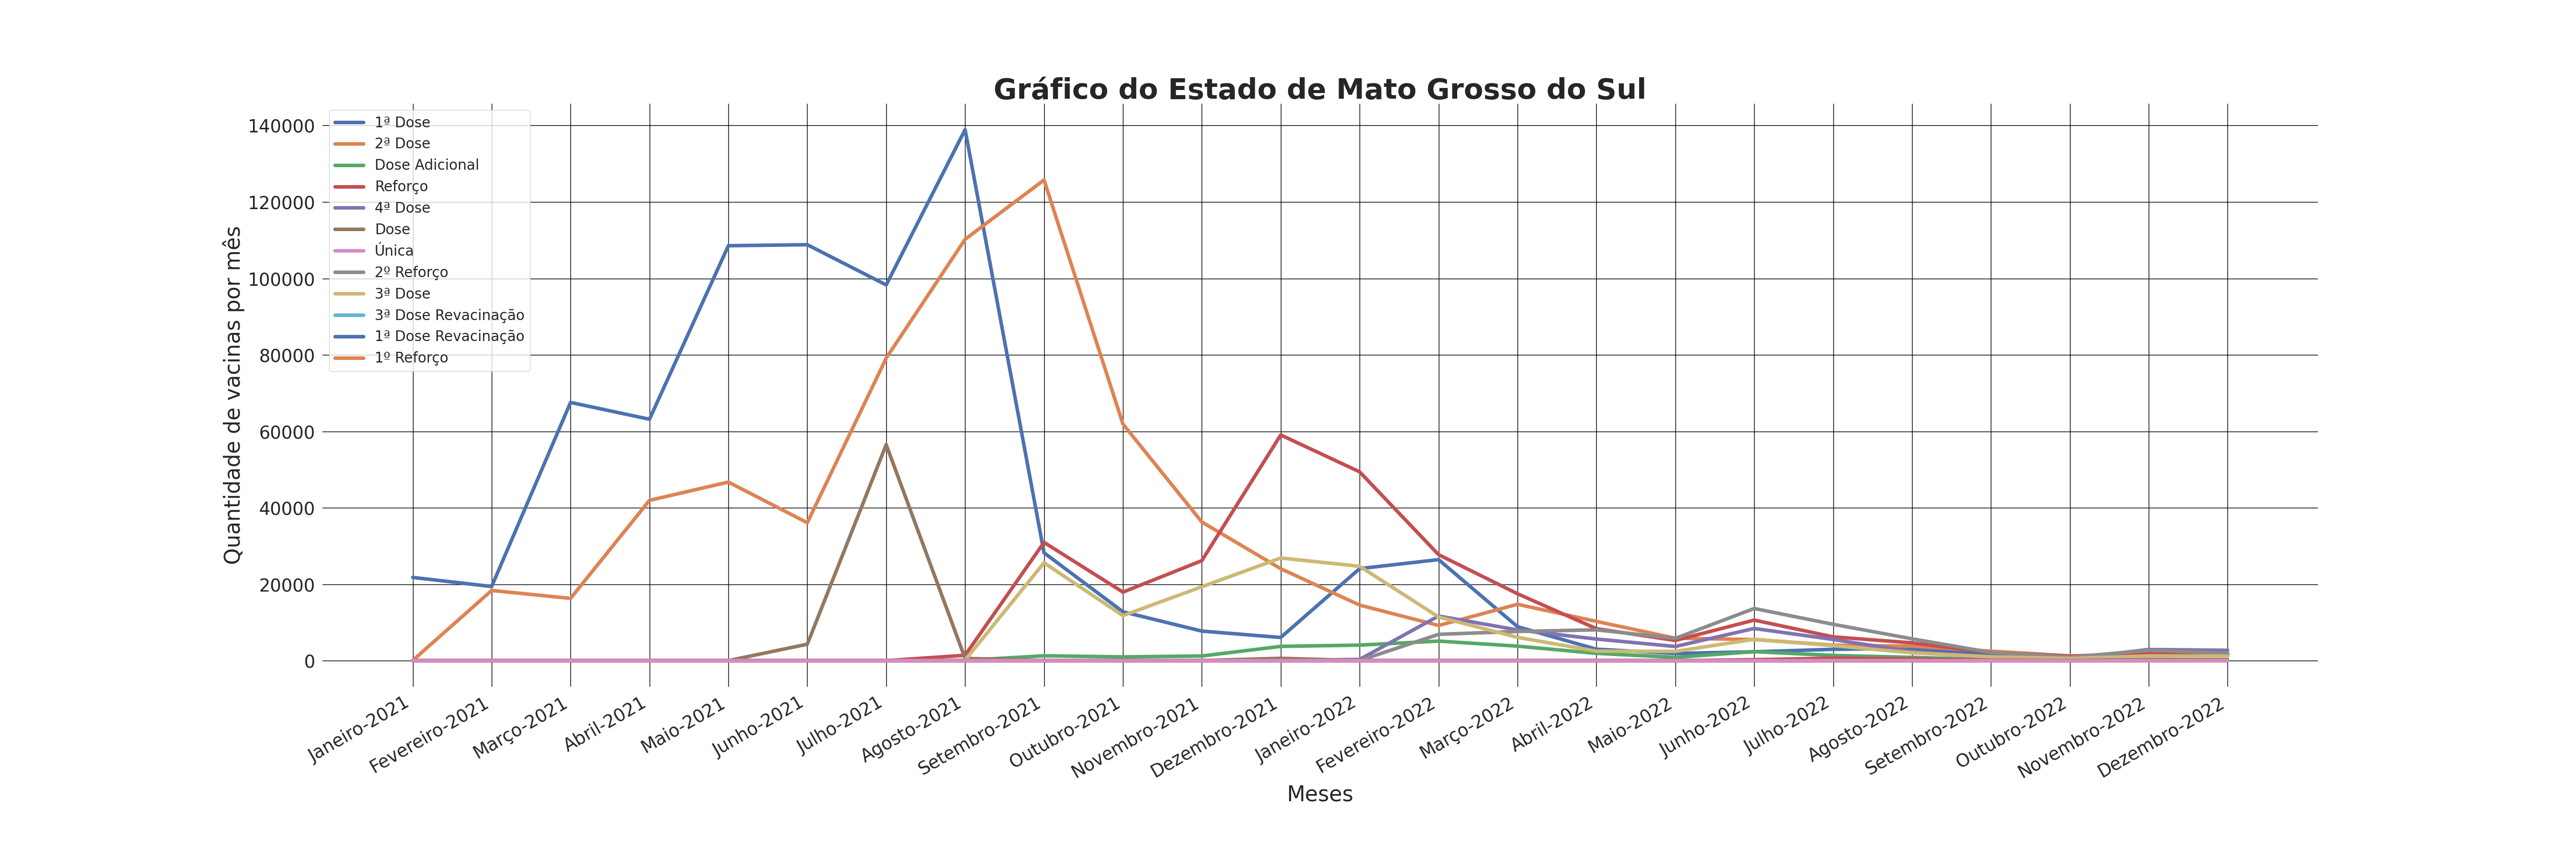
\includegraphics[width=.99\linewidth]{fig/Vacinação/2-MatoGrossodoSul.png}
        \caption{Quantidade de vacinas aplicadas por tipo de dose desde o início da vacinação naquele Estado até junho de 2022 no Estado de Mato Grosso do Sul.}
        \label{fig:my_label10}
    \end{figure}

    % \begin{figure}[!htp]
    %     \centering
    %     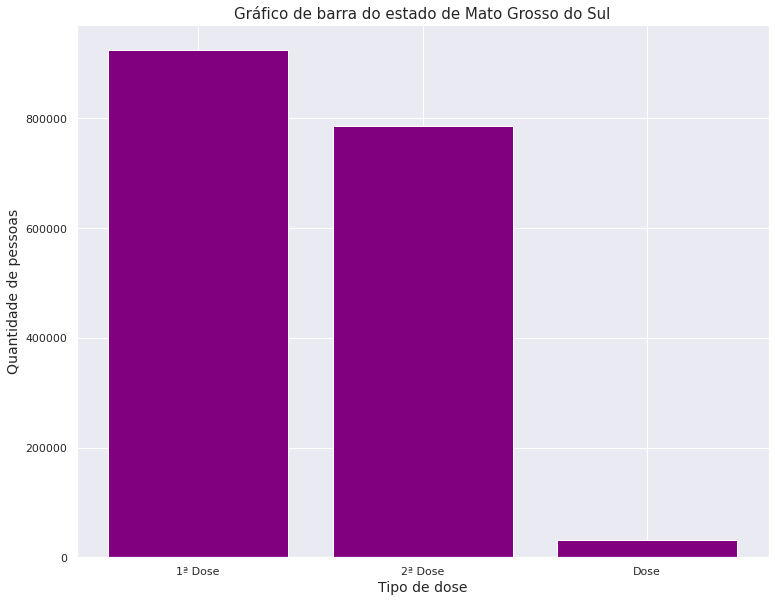
\includegraphics[width=.99\linewidth]{fig/Vacinação/3-MatoGrossodoSul.png}
    %     \caption{Quantidade de pessoas vacinadas na primeira, segunda e dose única no Estado de Mato Grosso do Sul.}
    %     \label{fig:my_label11}
    % \end{figure}
    
    % \begin{figure}[htp]
    %     \centering
    %     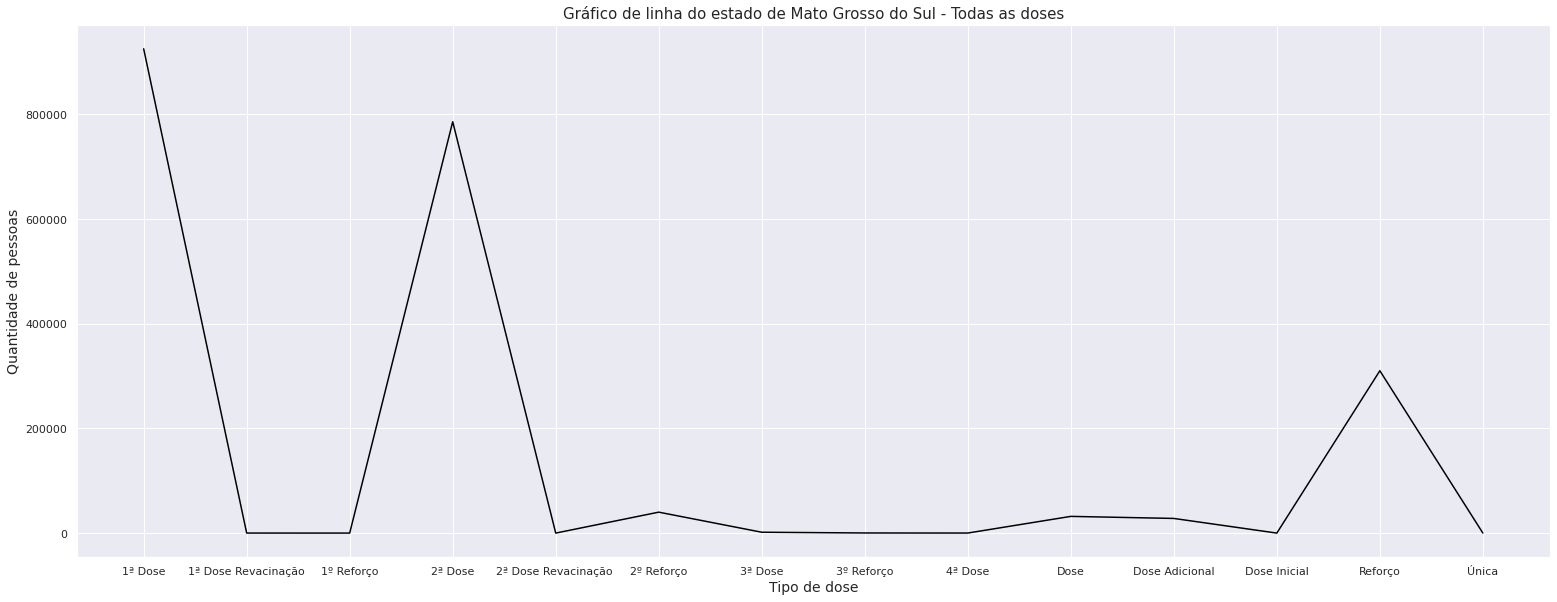
\includegraphics[width=.99\linewidth]{fig/Vacinação/4-MatoGrossodoSul.png}
    %     \caption{Quantidade de pessoas vacinadas em todas as doses no Estado de Mato Grosso do Sul.}
    %     \label{fig:my_label12}
    % \end{figure}

    \begin{figure}[!htp]
        \centering
        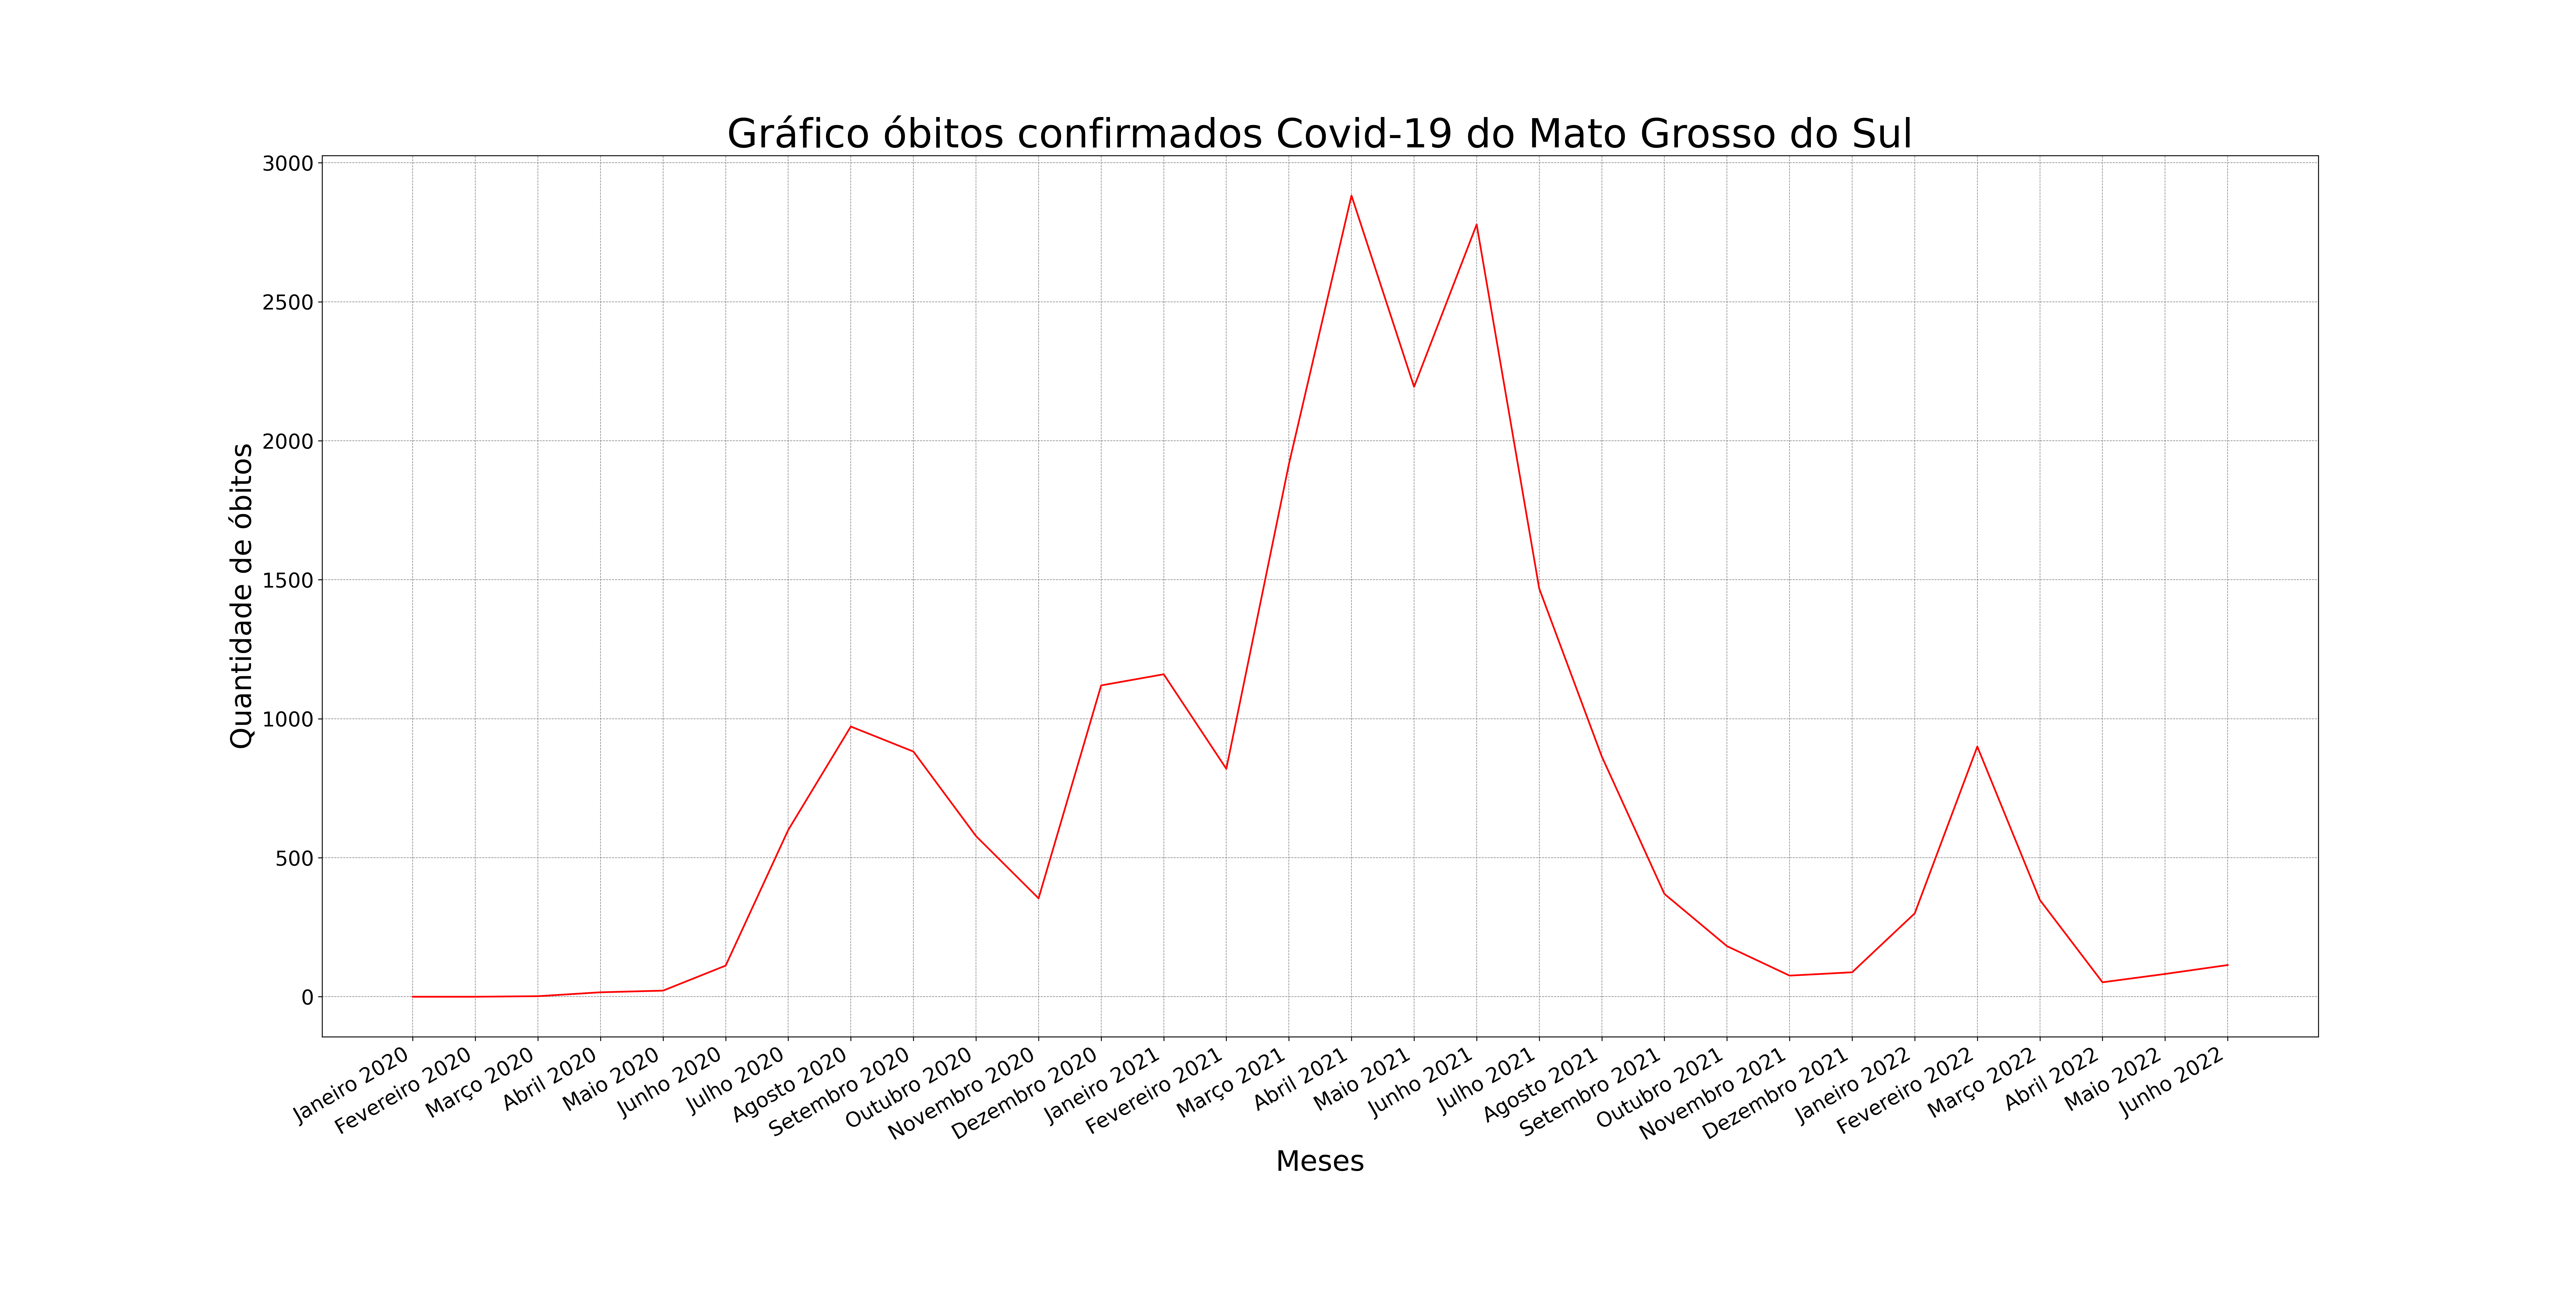
\includegraphics[width=.99\linewidth]{fig/Obitos/MS_Obitos.png}
        \caption{Quantidade de óbitos mensal no Estado de Mato Grosso do Sul.}
        \label{fig:my_label12}
    \end{figure}

\newpage
%\vspace{2cm}
\begin{center}
    \textbf{Distrito Federal}
\end{center}

    \begin{figure}[!htp]
        \centering
        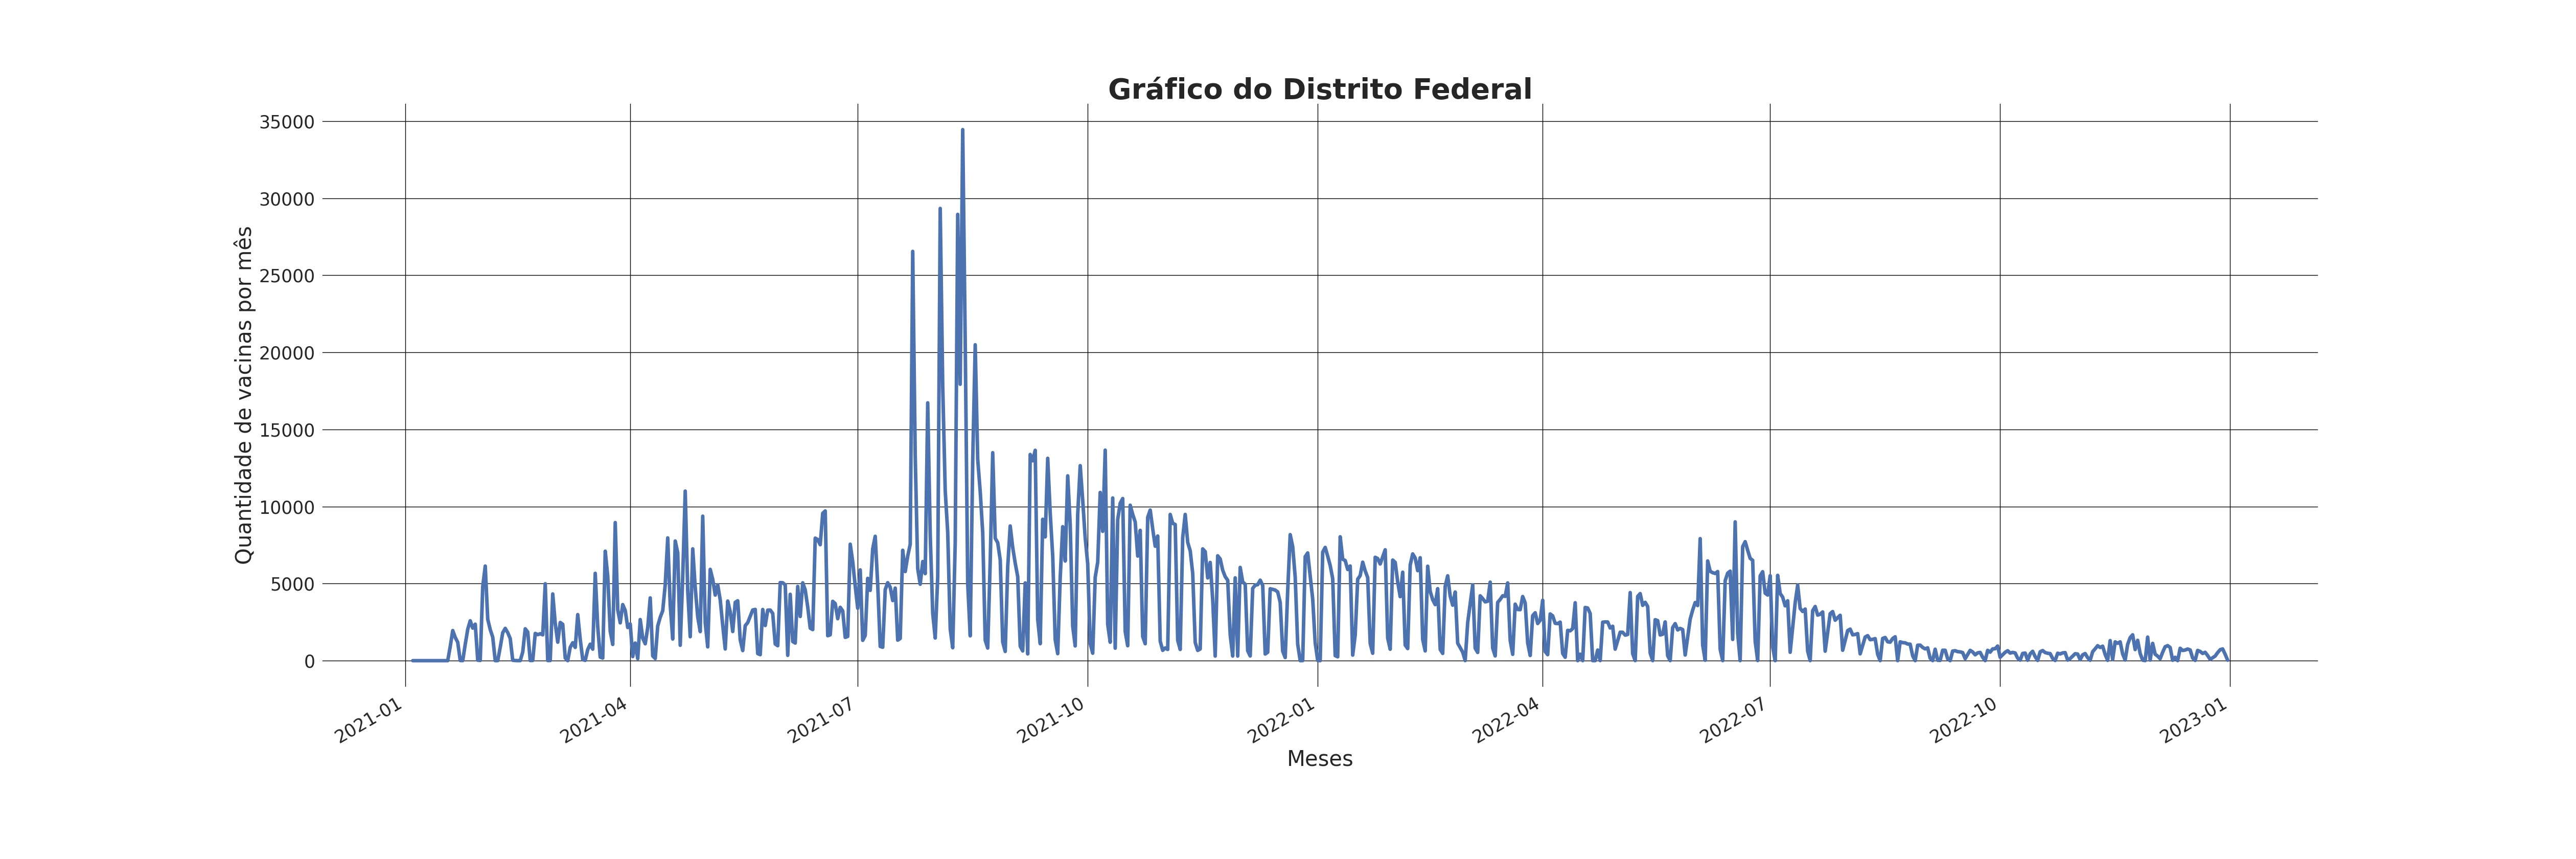
\includegraphics[width=.99\linewidth]{fig/Vacinação/1-DistritoFederal.png}
        \caption{Quantidade de vacinas aplicadas por mês no Distrito Federal.}
        \label{fig:my_label13}
    \end{figure}
    
    \begin{figure}[!htp]
        \centering
        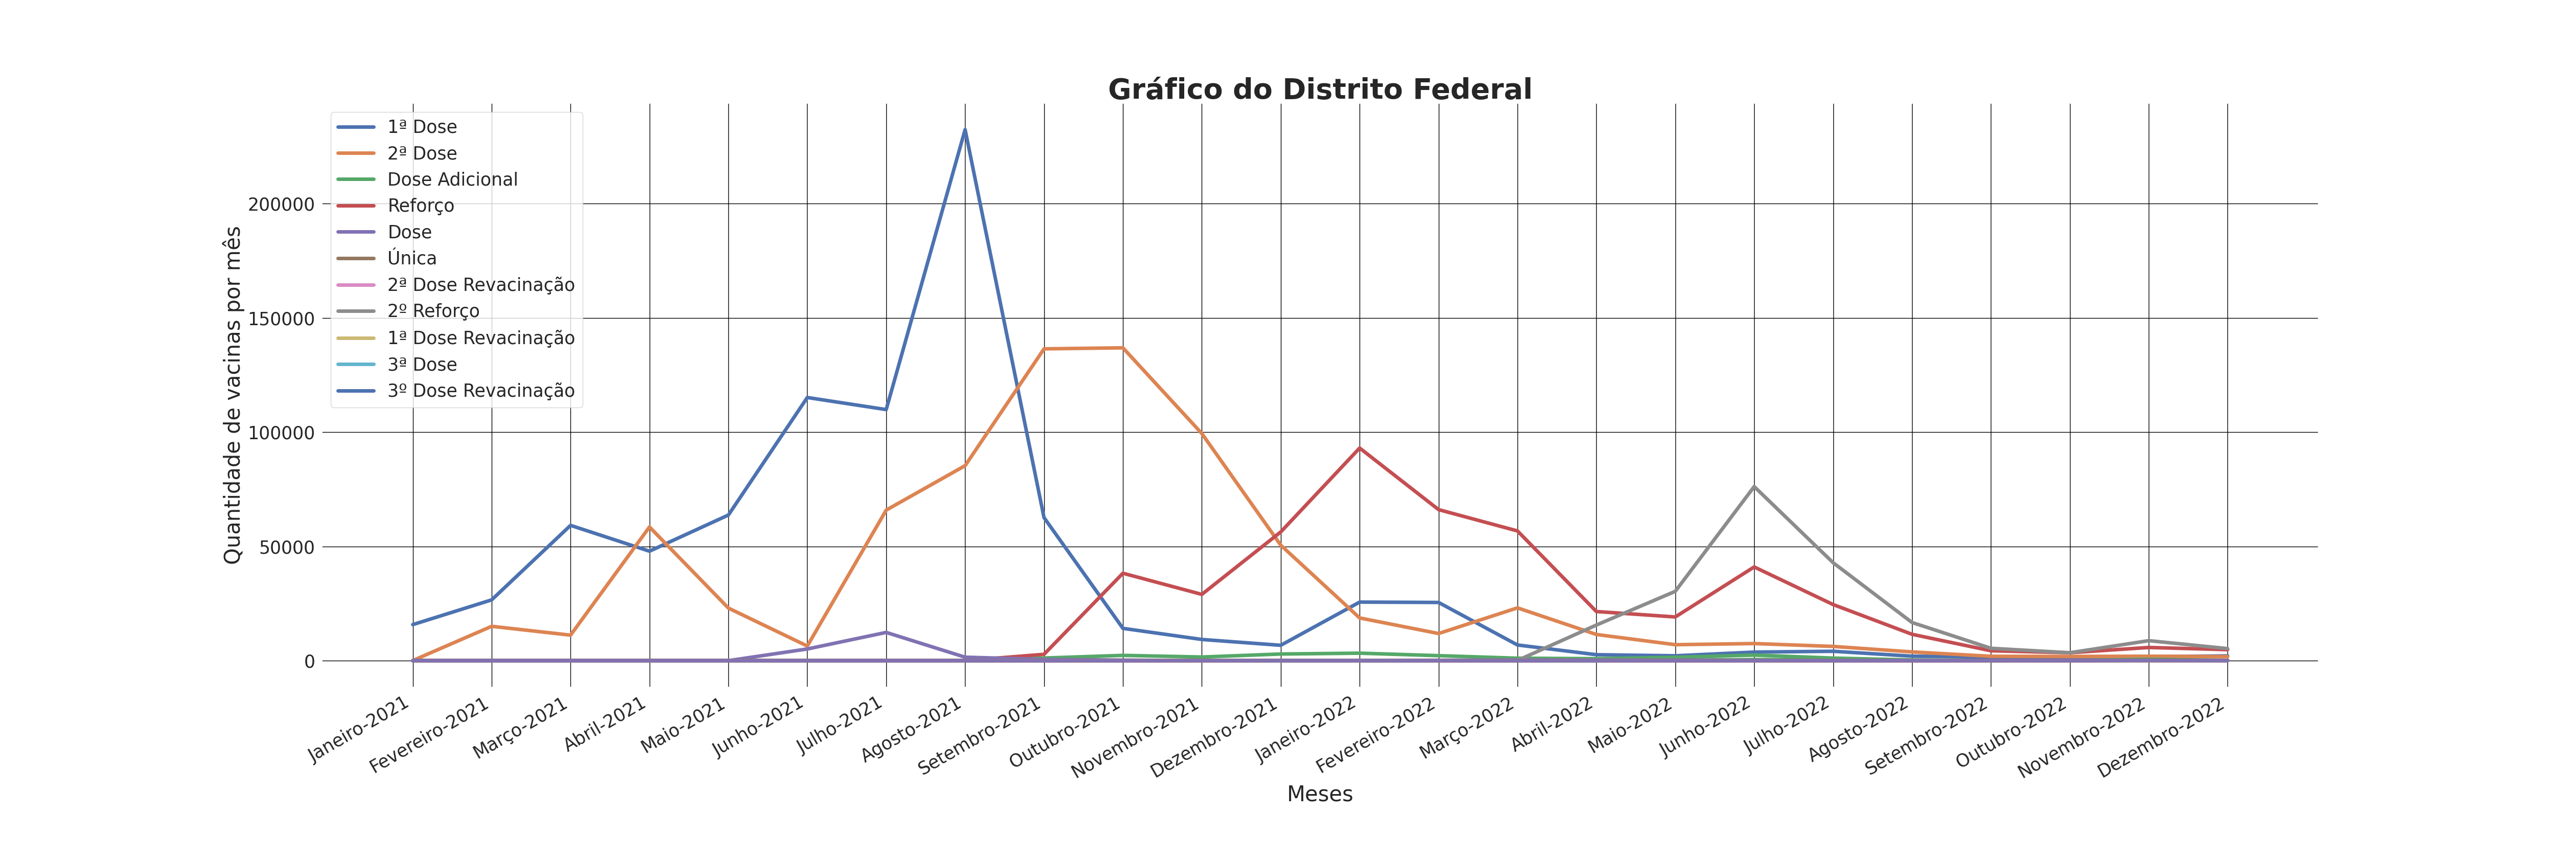
\includegraphics[width=.99\linewidth]{fig/Vacinação/2-DistritoFederal.png}
        \caption{Quantidade de vacinas aplicadas por tipo de dose desde o início da vacinação naquele Estado até junho de 2022 no Distrito Federal.}
        \label{fig:my_label14}
    \end{figure}

    % \begin{figure}[!htp]
    %     \centering
    %     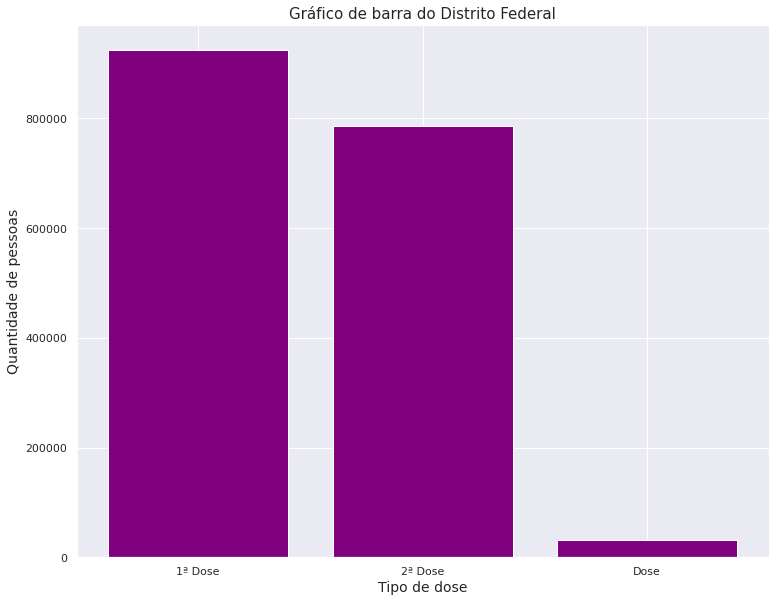
\includegraphics[width=.99\linewidth]{fig/Vacinação/3-DistritoFederal.png}
    %     \caption{Quantidade de pessoas vacinadas na primeira, segunda e dose única no Distrito Federal.}
    %     \label{fig:my_label15}
    % \end{figure}
    
    % \begin{figure}[htp]
    %     \centering
    %     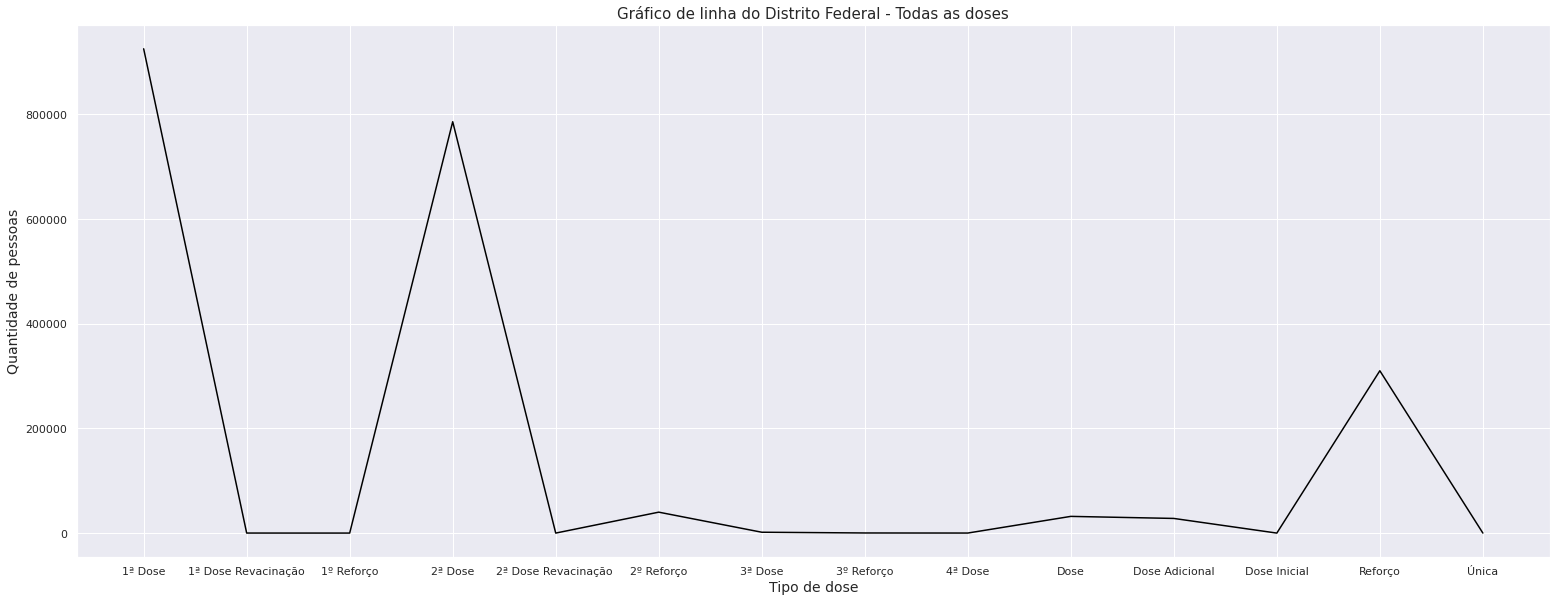
\includegraphics[width=.99\linewidth]{fig/Vacinação/4-DistritoFederal.png}
    %     \caption{Quantidade de pessoas vacinadas em todas as doses no Distrito Federal.}
    %     \label{fig:my_label16}
    % \end{figure}

    \begin{figure}[!htp]
        \centering
        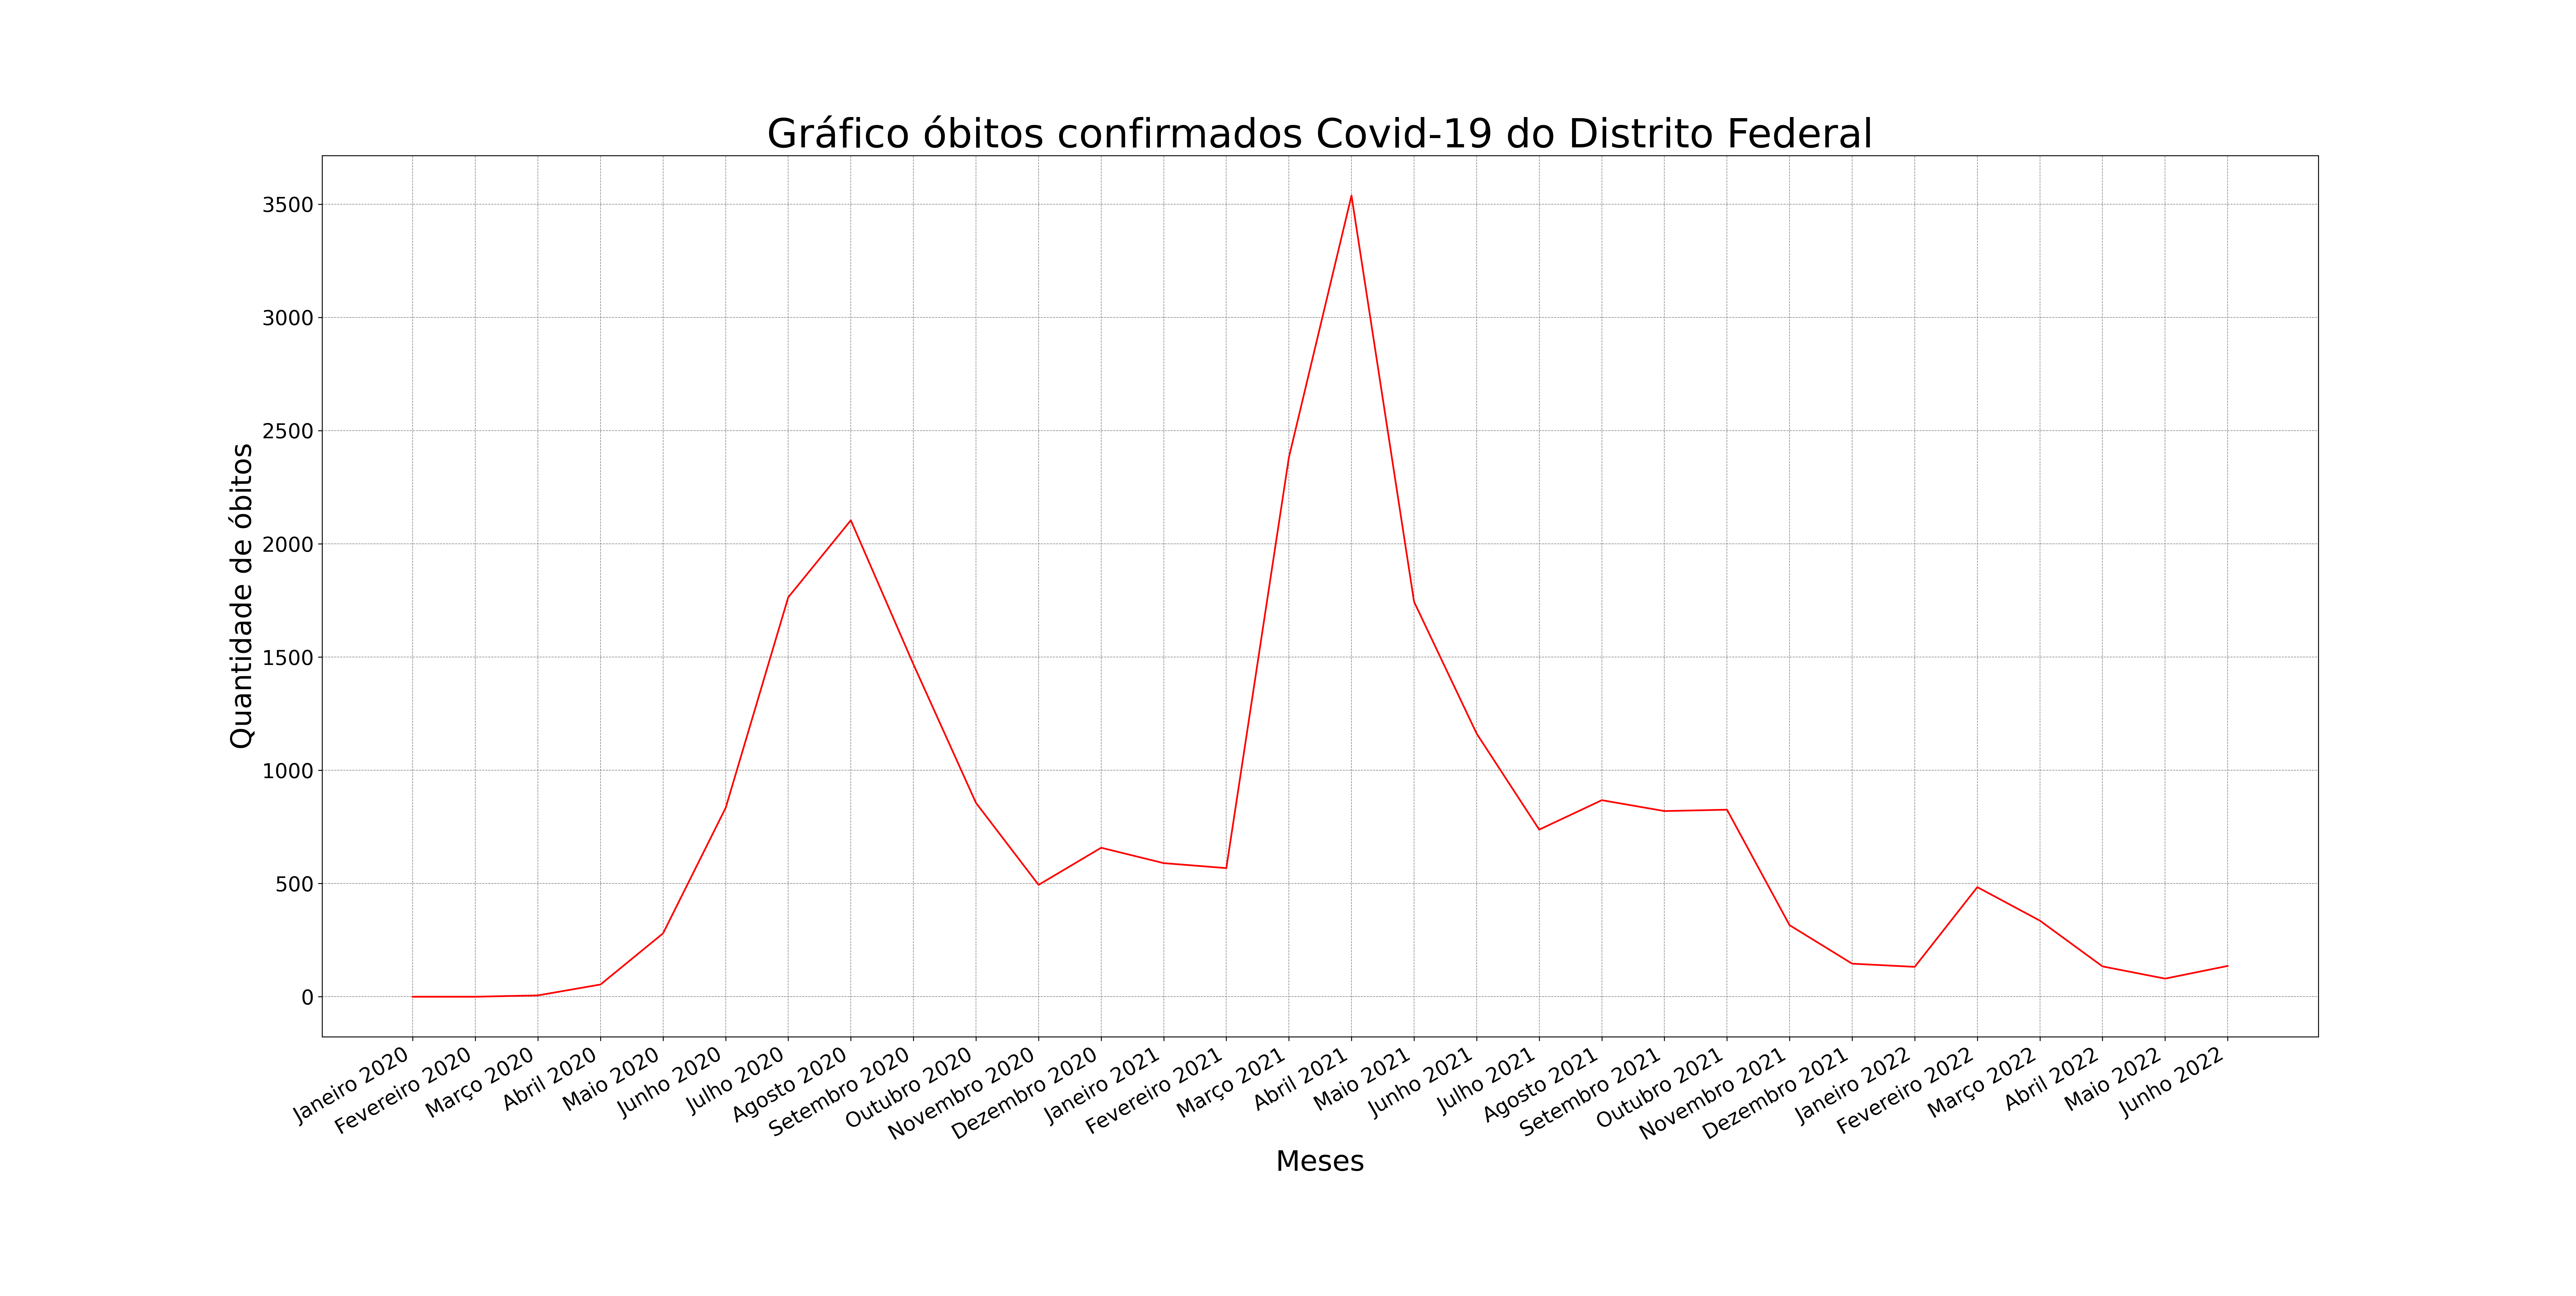
\includegraphics[width=.99\linewidth]{fig/Obitos/DF_Obitos.png}
        \caption{Quantidade de óbitos mensal no Distrito Federal.}
        \label{fig:my_label16}
    \end{figure}